%%%%%%%%%%%%%%%%%%%%%%%%%%%%%%%%%%%
% Basic formatting and settings
%%%%%%%%%%%%%%%%%%%%%%%%%%%%%%%%%%%
\documentclass[12pt,a4paper]{report}
\usepackage[utf8x]{inputenc}
\usepackage[IL2]{fontenc}
\usepackage{a4wide}
\usepackage[left=2cm, right=2cm, top=2.5cm, bottom=2.5cm]{geometry}

%%%%%%%%%%%%%%%%%%%%%%%%%%%%%%%%%%%
% Include required packages
%%%%%%%%%%%%%%%%%%%%%%%%%%%%%%%%%%%
\usepackage{amsmath,amssymb,amsthm}
\usepackage[usenames]{color}
\usepackage{nicefrac}
\usepackage{verbatim}
\usepackage{graphicx}
\usepackage{enumitem}
\usepackage{setspace}
\usepackage{tabularx}
\usepackage{listings}
\usepackage[section]{placeins}

\usepackage[pdftex,bookmarks=true,colorlinks,linkcolor=blue,urlcolor=blue,unicode]{hyperref}
\hypersetup{pdftitle=ODCleanStore}

%%%%%%%%%%%%%%%%%%%%%%%%%%%%%%%%%%%
% Additional formatting settings
%%%%%%%%%%%%%%%%%%%%%%%%%%%%%%%%%%%

%\pagestyle{plain}
\pagestyle{headings}
\linespread{1.1}
\setcounter{secnumdepth}{3}
\setcounter{tocdepth}{2}

%%%%%%%%%%%%%%%%%%%%%%%%%%%%%%%%%%%
% Include macro definitions and package settings
%%%%%%%%%%%%%%%%%%%%%%%%%%%%%%%%%%%

%%%%%%%%%%%%%%%%%%%%%%%%%%%%%%%%%%%
% Indent settings for paragraphs, itemize and enumerate environment
%%%%%%%%%%%%%%%%%%%%%%%%%%%%%%%%%%%
\setitemize{noitemsep,topsep=2pt,leftmargin=30pt}
\setenumerate{noitemsep,topsep=2pt,leftmargin=30pt}
\setdescription{style=sameline}
%\setlength{\parindent}{0pt} % nastavuje odsazení prvniho radku
%\setlength{\parskip}{1.2ex plus 0.5ex minus 0.2ex} % odstup mezi odstavci

\newcommand{\moreindent}{\addtolength{\leftskip}{1.8em}}
\newcommand{\lessindent}{\addtolength{\leftskip}{1.8em}}
\newcommand{\suppressgaps}{\setlength{\parskip}{0pt}}

%%%%%%%%%%%%%%%%%%%%%%%%%%%%%%%%%%%
% Shortcuts for math mode
%%%%%%%%%%%%%%%%%%%%%%%%%%%%%%%%%%%
\newcommand{\coloneqq}{\mathrel{\mathop:}=}
\renewcommand{\O}{{\mathcal{O}}}
\newcommand{\etc}[2]{#1_1,\ldots,#1_#2}
\def\<#1>{\leavevmode\hbox{\it #1\/}} % usage: \<variable>

%%%%%%%%%%%%%%%%%%%%%%%%%%%%%%%%%%%
% Other shortcuts and style commands
%%%%%%%%%%%%%%%%%%%%%%%%%%%%%%%%%%%
\newcommand{\quot}[1]{``#1''}
\newcommand{\code}[1]{\texttt{#1}}
\newcommand{\varcode}[1]{\textit{\textless #1\textgreater}}
\newcommand{\vartext}[1]{\textit{#1}}
\newcommand{\tab}{\rule{30pt}{0pt}}
\newcommand{\term}[1]{\textit{#1}}
\newcommand{\todo}[1]{}
\newcommand{\importantterm}[1]{\textbf{#1}}

% These macros use a dirty trick to persuade LaTeX to typeset chapter headers
% more readably and not to leave plenty of space above them.
\makeatletter
\def\@makechapterhead#1{
  {\parindent \z@ \raggedright \normalfont
   \Huge\bfseries \thechapter. #1
   \par\nobreak
   \vskip 20\p@
}}
\def\@makeschapterhead#1{
  {\parindent \z@ \raggedright \normalfont
   \Huge\bfseries #1
   \par\nobreak
   \vskip 20\p@
}}
\makeatother

% Chapter that is not numbered but included in the contents
\def\chapwithtoc#1{
\chapter*{#1}
\addcontentsline{toc}{chapter}{#1}
} 

\newenvironment{enumeratei}
	{
		\begin{enumerate}
		\renewcommand{\labelenumi}{(\textit{\roman{enumi}})}
	}
	{
		\end{enumerate}
	}

\newenvironment{glossarylist}
	{\begin{description}[style=nextline,itemsep=8pt]}
	{\end{description}}

\newenvironment{configlist}
	{\begin{description}[style=nextline,font=\ttfamily]}
	{\end{description}}

\newenvironment{dirlist}
	{\begin{description}[style=sameline,font=\ttfamily]}
	{\end{description}}
	
%%%%%%%%%%%%%%%%%%%%%%%%%%%%%%%%%%%
% Package settings
%%%%%%%%%%%%%%%%%%%%%%%%%%%%%%%%%%%%

% lstlistings environment
% Defines a custom trivlisting environment
\lstset{basicstyle=\ttfamily\footnotesize,columns=flexible,
  frame=lines,float=ht,captionpos=b,aboveskip=1.5\bigskipamount}
\lstnewenvironment{trivlisting}
  {\lstset{basicstyle=\ttfamily,aboveskip=\medskipamount,frame=none}}
  {}

%%%%%%%%%%%%%%%%%%%%%%%%%%%%%%%%%%%
% Document-specific commands
%%%%%%%%%%%%%%%%%%%%%%%%%%%%%%%%%%%
\newcommand{\refusermanual}{User Manual\xspace}
\newcommand{\refadminmanual}{Administrator's \& Installation Manual\xspace}
\newcommand{\refprogrammersguide}{Programmer's Guide\xspace}
\newcommand{\configdefault}[1]{\newline\textit{Default value:}~\code{#1}}
\newcommand{\odcs}{ODCleanStore\xspace}
\newcommand{\reqparagraph}[1]{\paragraph{\textnormal{\textit{#1}}}}

%%%%%%%%%%%%%%%%%%%%%%%%%%%%%%%%%%%
% Aligned enumeration tables
%%%%%%%%%%%%%%%%%%%%%%%%%%%%%%%%%%%
\newcommand{\enumtable}[1]
{
	\begin{table}[!ht]
		\begin{tabularx}{\linewidth}{>{\textbf\bgroup}l<{\egroup}X}
			#1
		\end{tabularx}
	\end{table}
}

%%%%%%%%%%%%%%%%%%%%%%%%%%%%%%%%%%%
% Aligned field description tables
%%%%%%%%%%%%%%%%%%%%%%%%%%%%%%%%%%%
\newcommand{\fieldtable}[1]
{
	\begin{table}[!ht]
		\begin{tabularx}{\linewidth}{|>{\textbf\bgroup}l<{\egroup}|p{3cm}|X|}
			\hline
			\textnormal{Required} & Field & Description \\
			\hline \hline
			#1 \\
			\hline
		\end{tabularx}
	\end{table}
}


%%%%%%%%%%%%%%%%%%%%%%%%%%%%%%%%%%%
% Optionally disable use of images.
% Convenient for export to .dvi when the documents contain images not supported in plain latex
% Uncomment to disable images.
%%%%%%%%%%%%%%%%%%%%%%%%%%%%%%%%%%%
%\renewcommand{\includegraphics}[2][1]{}

\newcommand{\version}{0.3.6}
\newcommand{\documentname}{\refprogrammersguide}

\hypersetup{pdftitle=ODCleanStore -- \documentname}

\begin{document}

\title{ODCleanStore -- \documentname}

\begin{titlepage}
\begin{center}

\large
Charles University in Prague

\smallskip

Faculty of Mathematics and Physics

%\vspace{\stretch{1}}
%{\bf\Large SOFTWARE PROJECT}

\vspace{\stretch{3}}

\resizebox{0.5\linewidth}{!}{\bf\Huge ODCleanStore}

%\bigskip
%\resizebox{0.3\linewidth}{!}{Open Data store}

\vspace{\stretch{3}}
\begin{spacing}{1.5} 
{\bf\Huge \documentname}
\end{spacing}

\vspace{\stretch{1}}
Release \version\\
\today

\vspace{\stretch{15}}

\begin{tabular}{rl}

\textbf{Authors:} & Jan Michelfeit \\
& Du\v san Rychnovsk\'y\\
& Jakub Daniel\\
& Petr Jerman\\
& Tom\' a\v s Soukup\\
\noalign{\vspace{3mm}}
\textbf{Supervisor:} & RNDr. Tom\' a\v s Knap
\end{tabular}

\end{center}
\end{titlepage}

\newpage

\renewcommand{\contentsname}{Contents}
\tableofcontents
\bigskip

\newpage

%%%%%%%%%%%%%%%%%%%%%%%%%%%%%%%%%%%%%%%%%%%%%%%%%%%%%%%%%%%%%%%%%%%%%%%%%%%%%%

  % FE - popsat, že to je webová aplikace, dá se spouštět pod tomcatem, odkaz na install manual

%%%%%%%%%%%%%%%%%%%%%%%%%%%%%%%%%%%%%%%%%%%%%%%%%%%%%%%%%%%%%%%%%%%%%%%%%%%%%%

\chapter{Introduction}
\odcs is a~server application for management of Linked Data written in Java. It stores data in RDF, processes them and provides integrated views on the data.

This document serves as the main documentation for developers. It describes basic architecture, implementation, development process, used technologies and other important information relevant for people who want to participate in the development of \odcs.

\section{What is ODCleanStore}
\odcs accepts arbitrary RDF data and metadata through a SOAP webservice (\term{Input Webservice}). The data is processed by \term{transformers} in one of a~set of customizable \term{pipelines} and stored to a~persistent store (OpenLink Virtuoso database instance). The stored data can be accessed again either  directly through a SPARQL endpoint or through \term{Output Webservice}. Linked Data consumers can send queries and custom query policies to Output Webservice and receive (aggregated/integrated) RDF data relevant for their query, together with information about provenance and data quality. 

\section{Related documents}
More detailed information about \odcs from the perspective of a user or an administrator can be found in related documents \quot{\refusermanual} and \quot{\refadminmanual}. \refusermanual also contains definition of user roles, glossary of terms etc.

Other working documents related to development are located at the project's page at SourceForge\footnote{\url{https://sourceforge.net/p/odcleanstore/wiki/For\%20developers/}}. The Wiki tool at SourceForge is used for working documents, discussion of new features, description of testing scenarios etc. Not all pages are up-to-date, however, and this document is authoritative in case of conflicts.

%%%%%%%%%%%%%%%%%%%%%%%%%%%%%%%%%%%%%%%%%%%%%%%%%%%%%%%%%%%%%%%%%%%%%%%%%%%%%%
%\chapter{Requirements}
% todo
% features, interfaces, administration, future use
% motivace, ostatní existující řešení, v čem je to nové


%%%%%%%%%%%%%%%%%%%%%%%%%%%%%%%%%%%%%%%%%%%%%%%%%%%%%%%%%%%%%%%%%%%%%%%%%%%%%%
\chapter{ODCleanStore overview} 
An overview of how \odcs works is depicted on \figurename~\ref{fig:odcsInternal}.

\begin{figure}[htb]
    \centering
    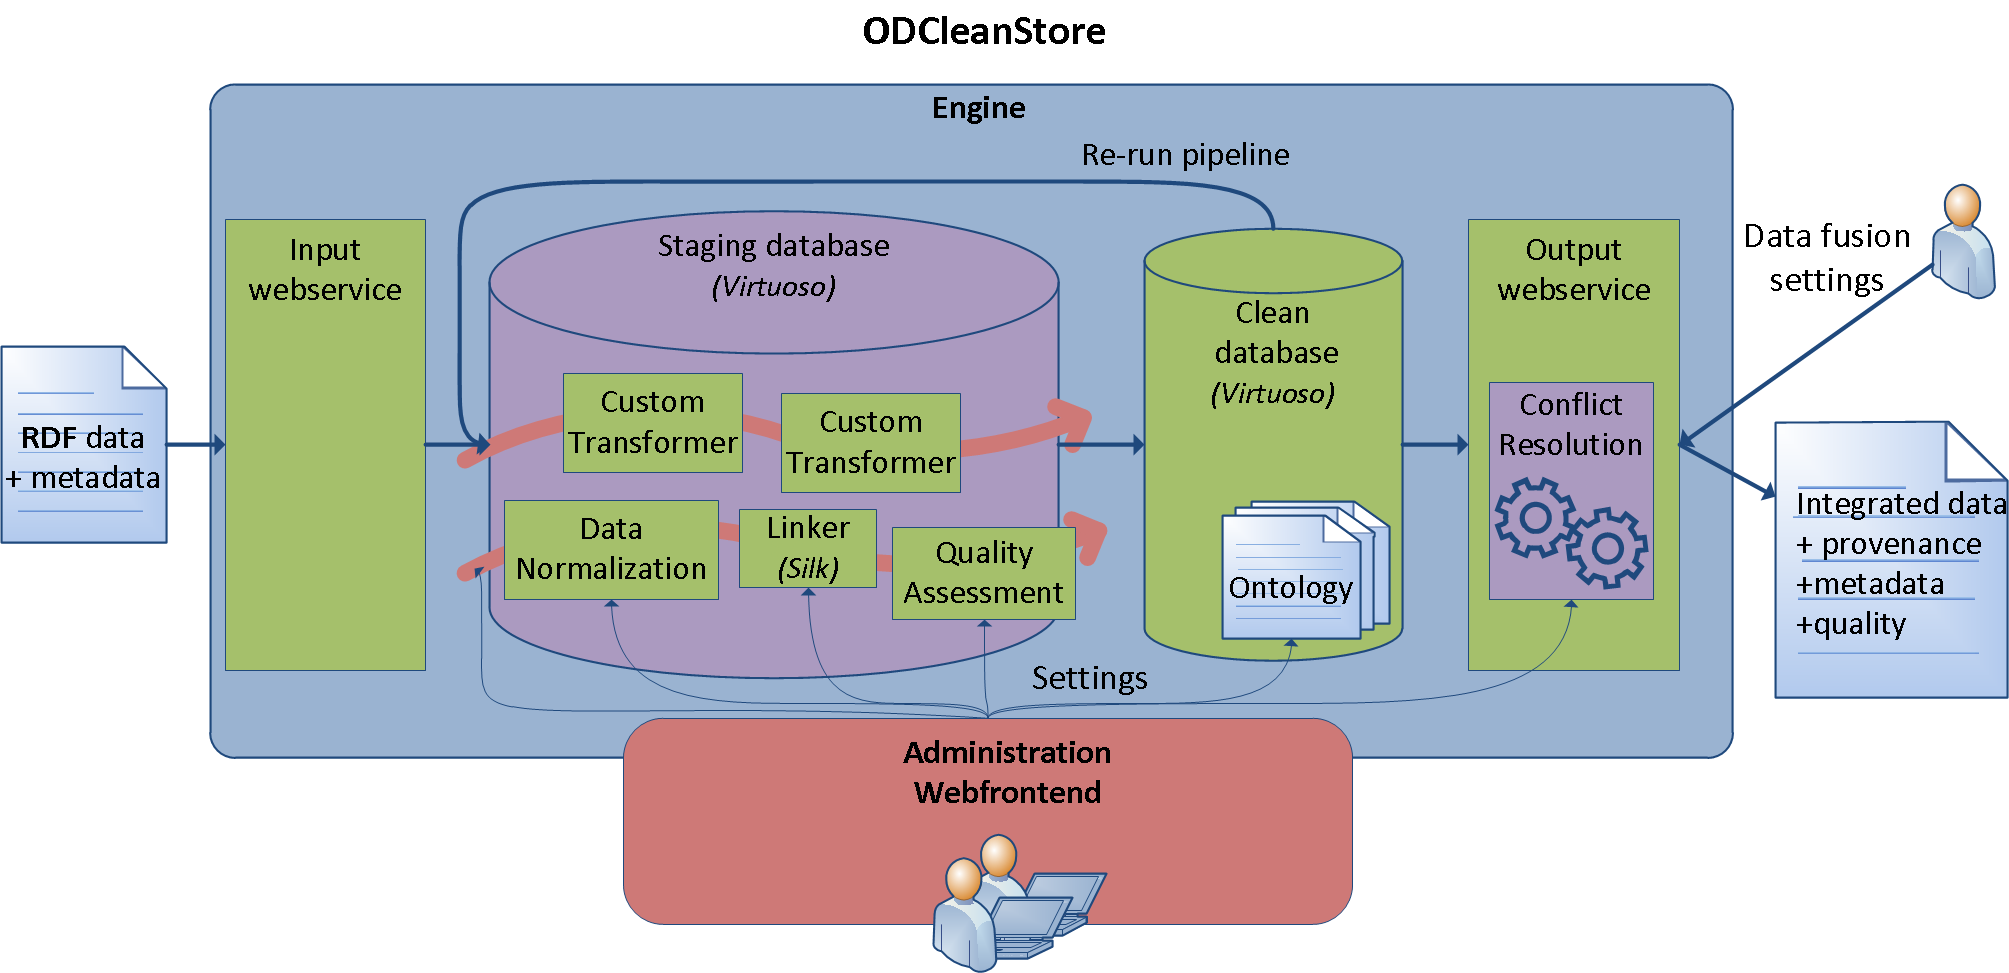
\includegraphics[width=\textwidth]{images/odcs-internal.png}
    \caption{Overview of ODCleanStore architecture}
	\label{fig:odcsInternal}
\end{figure}

The diagram lists all main functional units in \odcs:

\begin{itemize}
	\item \importantterm{Engine.}
		Engine runs the whole server part. It realizes all data processing and starts Input and Output Webservices.

		\begin{itemize}
			\item \importantterm{Input Webservice}. SOAP webservice that accepts new data and queues them for processing in the dirty database.
			\item \importantterm{Pipeline processing}. Processes queued data by running a series of transformers in a pipeline on it and moves the data to the clean database.
			\item \importantterm{Ouptut Webservice}. REST webservice for querying over data in the clean database.
		\end{itemize}
	\item \importantterm{Query Execution \& Conflict Resolution.}
		\QE retrieves all data and metadata relevant for a query asked via Output Webservice. Conflict Resolution then resolves conflicts in the retrieved data, including resolution of \code{owl:sameAs} links.
	\item Predefined transformers.
		Transformers used for data processing that are included by default in \odcs.
		\begin{itemize}
			\item \importantterm{Quality Assessment}. Estimates quality of data based on user-defined or generated rules.
			\item \importantterm{Data Normalization}. Transformations of data based on user-defined or generated rules.
			\item \importantterm{Linker}. Generates links (e.g. \code{owl:sameAs}) between resources in the processed data and contents of the clean database.
			\item Other transformers -- Other transformers such as Quality Aggregator, Blank Node Remover etc.
		\end{itemize}
	\item \importantterm{Administration Frontend.}
		Web application written in Java from which \odcs can be managed. In \FE, the user can define pipelines for data processing, rules for transformers, manage ontologies, Output Webservice settings etc.
\end{itemize}

Each of these parts will be described later in this document. In the source code, the components are divided into several maven projects described in Section \ref{sec:mavenBuild}.

\section{Important concepts}
\odcs is about data. More specifically, it works with data represented in RDF\footnote{\url{http://www.w3.org/TR/2004/REC-rdf-primer-20040210/}}. \odcs implements three tasks regarding data:

\begin{enumerate}
	\item Data processing
	\item Storing data
	\item Querying over stored data
\end{enumerate}

\subsection{Data Processing}
\label{sec:dataProcessing}
Data processing is realized by \term{transformers} that are applied to data being processed by Engine in a \term{pipeline}. A transformer can be any class implementing the \code{Transformer} interface but typically it only manipulates (change, add, delete) processed data in database. Several transformers ship with \odcs, such as \QA, \OI or \DN.

It is important to distinct between a \term{transformer} and \term{transformer instance}. By \term{transformer}, we mean the Java class which implements the \code{Transformer} interface and is registered in ODCleanStore administration (managed by users in role Administrator). \term{Transformer instance} is assignment of such transformer to a pipeline. For example, the \QA transformer is registered in ODCleanStore by default. The user can create two pipelines and assign the \QA transformer to each of them, thus creating two transformer instances.

Some transformers can be configured in \FE by \term{rules}. In general, these rules are grouped to \term{rule groups}. Rule groups can be then assigned to transformer instances.

See also Section \ref{sec:dataLifecycle} \nameref{sec:dataLifecycle}.

\subsection{Storing Data}
Data are stored using Open Link Virtuoso RDF database. Two instances of this database are used for every deployment of \odcs:

\begin{itemize}
	\item \term{Dirty (staging) database} -- contains data that are currently being processed. Contents of this instance is not directly visible for data consumers (users in role USR).
	\item \term{Clean database} -- contains already processed data that are accessible through the Output Webservice to data consumers (users in role USR).
\end{itemize}

\subsection{Querying over Stored Data}
Querying over stored data is realized by Output Webservice which supports several types of queries (see \refusermanual). For retrieval of results and resolving conflicts, Output Webservice uses components \QE (Section \ref{sec:QE}) and Conflict Resolution (Section \ref{sec:CR}).

\subsection*{}

See also Glossary in Appendix \ref{chap:glossary} for explanation of important concepts.

\section{Data Lifecycle}
\label{sec:dataLifecycle}

The lifecycle of data inside \odcs is as follows:

\begin{enumerate}
  \item RDF data (and additional metadata) are accepted by Input Webservice and stored as a~named graph to the {dirty database}. Data can be uploaded by any third-party application registered in \odcs.
  \item Engine successively processes named graphs in the dirty database by applying a~pipeline of transformers to it; the applied pipeline is selected according to the input metadata.
  \item Each transformer in the pipeline may modify the named graph or attach new related named graphs (such as a named graph with mappings to other resources or results of quality assessment).
  \item When the pipeline finishes, the augmented RDF data are populated to the {clean database} together with any auxiliary data and metadata created during the pipeline execution.
  \item Data consumers can use Output Webservice to query data in the clean database. Output Webservice provides several basic types of queries -- URI query, keyword and named graph query; in addition, metadata about a~given named graph can be requested. The response to a~query consists of relevant RDF triples together with their provenance information and quality estimate. The query can be further customized by user-defined conflict resolution policies.\\
	Data in the clean database can be also queried using the SPARQL query language. While SPARQL queries are more expressive, there is no direct support for provenance tracking and quality estimation. 
  \item When transformer rules change, the administrator may choose to re-run a~pipeline on data already stored in the clean database. Copy of this data is created in the dirty database where it is processed by the pipeline. After that, the processed version of data replaces the original in the clean database.
\end{enumerate}

%%%%%%%%%%%%%%%%%%%%%%%%%%%%%%%%%%%%%%%%%%%%%%%%%%%%%%%%%%%%%%%%%%%%%%%%%%%%%%
\chapter{Implementation}
\section{Architecture}

\subsection{Architecture Evolution}
The architecture that is depicted on \figurename~\ref{fig:odcsInternal} was chosen for several reasons.

First, the division into components is natural with regard to the original specification of the software project. All important components are included and we have also kept other concepts, such as two dataspaces for clean and dirty data, or the flexibility of data-processing pipeline.

Second, the selected architecture allowed a clear division of work and enabled a relative independence of each component.

Third, it is a result of a long process of analysis. From the initial vision and  requirements specification, which suggested an abstract concept of tranformers run in arbitrary order on data, we extracted several most important cases of transformers that were tightly bound to the system and could run only in a fixed order, only to generalize them back to transformers with a~very simple interface and flexible pipelines.

\subsection{Usage Assumptions}
The architecture, and in particular the way editing of pipelines and rules  in \FE is solved, is based on several assumptions about how \odcs will be used. In this section we try to give an overview of these assumptions.

\begin{itemize}
	\item Data sent to Input Webservice are expected to be reasonably small. \odcs is designed to technically handle even very large data, however, for example results of \QA may not be relevant for a large graph because a small mistake in several values would decrease the \QA score for the whole large dataset. Motivation for this assumption is based on planned integration with project Strigil (see related work in Chapter \ref{chap:relatedWork}).
	\item Pipeline creators understand the data for which their pipelines are created but not necessarily understand data for pipelines created by other users. For this reason, editing is limited to an author of a pipeline so that a pipeline creator's pipelines cannot be broken by other users without his knowledge.
	\item The team of people working with a deployed \odcs may be decentralized and open, for example students using a shared instance for their own projects. For that reason the system should be robust, permissions should be reasonably limited, a single user shouldn't be able to block the whole system and there should be a possibility to correct wrong configuration for administrators.
	\item We expect that pipeline creators will usually be  data producers  using the Input Webservice at the same time. These users need some technical knowledge -- at least they should understand RDF and SPARQL. On the other hand, data consumers need not be technically skilled or understand RDF, even though it is benefitial. Data for these users may be presented in the HTML output of Output Webservice or through a third-party interface.
\end{itemize}


\subsection{Architectural Features}

\subsubsection{Components}
\odcs consists of several components that are (mostly) loosely-coupled only through a simple interface specified in advance. This made it easy divide tasks among developers and enabled them to work independently.

\subsubsection{Internal Interfaces}
In order to minimize interfaces between parts of \odcs, to minimize system requirements and to make the system more robust, we decided to prefer communication through data shared in database.

There is no direct interface between Engine and \FE, but the \FE saves all configuration to a relational database from which the Engine can retrieve it. This enbles updates of settings in transactions, prevents synchronization issues and enables the two parts to run completely independendently (even on separate machines).

Transformers run in a pipeline are isolated and don't know about each other. Instead of passing data to be transformed through an interface in memory, only the names of named graphs where data are stored are passed to each transformer. This enables to write transformers that are oblivious to \odcs as much as possible and only need to work with data by manipulating the database. Also, it gives transformers the full power of the SPARQL/SPARUL language. Although we should note that in practice, the transformer implementation may be tied with the use of Virtuoso as the underlying database, this is not such a downside because Virtuoso is one of the most popular RDF databases.

\subsubsection{Extensibility}
The main point of extensibility are custom transformers (see Section \ref{sec:customTransformers}). Because one only needs to implement a simple interface and is not bound to any specific technology (except of the limitations of the underlying Virtuoso database), transformers provide a very powerful way how to extend data processing capabilities.

\subsubsection{Interoperability}
The external interfaces are implemented using standard technologies (SOAP for Input Webservice, REST for Output Webservice) and standard formats (RDF/XML, Turtle/Notation3). This should minimize the effort for integration with third-party applications communicating with \odcs. We also provide a Java library for accessing the Input Webservice to futher minimize the effort.

\subsubsection{Used Technologies}
The choice of Java for implementation and Virtuoso as the underlying database ensure platform independence.

Since Java is a very wide-spread language, \odcs can be extended with minimum effort for learning new technologies (e.g. when adding new transformers).

\subsubsection{Scalability}
 Although currently the Engine is processing data sequentially, it is designed for parallel processing in the future. It could even be extended to work in a distributed manner on several machines.

 Most of the work the Input Webservice has is with data processing in pipelines. Since pipelines can run independently, each Engine instance could even use a dedicated database instance for dirty data.

 On the other hand, the Output Webservices uses the clean database in a read-only manner and thus could be also deployed on several database instances if database replication is put in place.

\section{Other Requirements}
The assignment of the project impose several additional requirements. This section lists how they were satisfied.

\reqparagraph{It should be easy to incorporate other components, such as a component computing popularity of the data sources.} This requirement is satisfied with the introduction of custom transformers.

\reqparagraph{The application will involve graphical user interface enabling management of all kinds of policies etc.} \FE enables management of all relevant settings. In addition, several user roles are supported and user accounts can be managed from \FE.

\reqparagraph{The application will run at least on Windows 7, Windows Server 2008, Linux.} \odcs requires Java Runtime Environment and Virtuoso installation, both supported on all of the listed platforms. \odcs has been tested on Windows 7, Windows Server 2008 and Debian distribution of Linux.

\reqparagraph{Application will be freely available under Apache Software License.} \odcs is published under the required license (see \refadminmanual) and source codes available at a public repository at SourceForge.net

\section{Used Technologies}

\subsection{Implementation Language}
The chosen language for implementation is Java. The reason is that there are many libraries and tools required for implemenation accessible in Java, it enables platform independence (one of the requirements on \odcs) and also it is very wide-spread so that developers don't need to learn a new syntax.

\subsection{Database}
Openlink Virtuoso\footnote{\url{http://virtuoso.openlinksw.com/}} is used as the underlying data store. It is the most popular RDF storage with a solid support. Both a commercial version and Open Source edition\footnote{\url{http://virtuoso.openlinksw.com/dataspace/dav/wiki/Main/}} exists.

RDF data store provided by Virtuoso supports reasoning, most notably \code{owl:sameAs} link resolution, which proved essential for Query Execution/Conflict Resolution components. Virtuoso also provides a relational database which relieves us from the need of another database for that purpose.

The downside is somewhat buggy behavior (especially SPARQL query parsing) and lack of working support for transactions with RDF data.

\subsection{Administration Frontend}
Apache Wicket\footnote{\url{http://wicket.apache.org/}} is used for implemenation of the \FE. It is a component system for writing web applications in Java. Advantages are proper mark-up and logic separation, POJO data model and rapid development of this particular type of web application. Wicket was also chosen by our sister project Strigil\footnote{\url{http://strigil.sourceforge.net/}} so a more tight integration of the two tools may be possible in the future.

Spring\footnote{\url{http://www.springsource.org/}} is used for simplified access to the relational database and transaction management. Use of Hibernate\footnote{\url{http://www.hibernate.org/}} for the DAO layer was rejected because of integration problems with Wicket.

\subsection{Libraries}
\subsubsection*{Jena}
Apache Jena\footnote{\url{http://jena.sourceforge.net/}} is a library for manipulation with RDF data. It supports represenation of RDF data in memory, parsing, loading and updating of RDF models. In \odcs, it is used mainly for representation of RDF triples (quads) and serialization of RDF, because other features proved problematic when used with large data.

We chose Jena over its alternative Sesame\footnote{\url{http://www.openrdf.org/}} because it supports working with named graphs through NG4J and we had previous experience with it.

\subsubsection*{NG4J}
NG4J\footnote{\url{http://wifo5-03.informatik.uni-mannheim.de/bizer/ng4j/}} extends Jena with named graphs API.

\subsubsection*{Restlet}
Restlet\footnote{\url{http://www.restlet.org}} is an open source lightweight RESTful web framework for Java. Output Webservice is built on Restlet.

\subsubsection*{SLF4J}
SLF4J\footnote{\url{http://www.slf4j.org/}} is a flexible and efficient library used for logging. 

\subsection{Development Tools}
\subsubsection*{Maven}
Apache Maven\footnote{\url{http://maven.apache.org/}} is used as the build tool. It was chosen over Apache Ant because Maven saves work with its many available plugins (such as Maven Jetty Plugin) and offers simple management of dependencies.

\subsubsection*{Git}
Git is used as the version control system. We used it because it enables simple manipulation with branches and merging but most importantly it is less dependent on a central server whose potential unavailability was identified as a potential risk.



%%%%%%%%%%%%%%%%%%%%%%%%%%%%%%%%%%%%%%%%%%%%%%%%%%%%%%%%%%%%%%%%%%%%%%%%%%%%%%
\chapter{Setting up Development Environment}

\section{Quick Start}
\subsection{Tools}
	In order to to prepare environment for building \odcs, first make sure to have installed all necessary tools:

\begin{itemize}
	\item Java Development Kit\footnote{\url{www.oracle.com/technetwork/java/javase/downloads/}} version 6 or newer
	\item Git version control system\footnote{\url{http://git-scm.com/}}
	\item Apache Maven\footnote{\url{http://maven.apache.org/}}
\end{itemize}

Also, make sure you have all the binaries used in the following steps on your classpath. 

\subsection{Obtaining sources} 
\odcs sources are hosted at SourceForge.\footnote{\url{http://sourceforge.net/p/odcleanstore/code/}} Use git to check out the sources:

\begin{verbatim}
      git clone git://git.code.sf.net/p/odcleanstore/code odcleanstore-code
\end{verbatim}

The above command will create a local clone of the repository in \code{odcleanstore-code} directory.

\subsection{Building binaries}
Move to directory \code{odcleanstore} within your local clone of the repository which contains the root maven project (\code{pom.xml}). Then build the project using maven:

\begin{verbatim}
      cd odcleanstore-code/odcleanstore
      mvn clean package install
\end{verbatim}

After that, Engine binaries can be found in directory \code{odcleanstore/engine/target} and the WAR file of \FE at \code{odcleanstore/webfrontend/target}. Now you can deploy the application as described in \refadminmanual. \todo{jestli tam bude jenom popis instalatoru, mel by se rucni deploy popsat tady a pridat referenci na instalaci Virtuosa}

\section{Repository structure}
\subsection{Branches}
There are several branches in the git repository. The latest development version of is on branch \code{master}. Then there are release branches for each release named \code{release-0.1.x}, \code{release-0.2.x} etc. which contain stable versions for  releases  packages. Each commit that was used to prepeare a release package is labeled with a tag \code{release}-\varcode{version}. Finally, there are feature branches prefixed with \code{feature-}.

Common development takes place on branch \code{master}. New feature branches are created for features that may or may not be accepted or that need time to be finished before they are applied to \code{master}. When whey are finished, they are merged to \code{master} and the branch may be removed in time. Release branches stem from \code{master} for every new major release. Fixes and modifications for minor releases take place on release branches and may be merged from/to \code{master}.

\subsection{Directory structure}
This is an outline of directory structure in the git repository:

\begin{dirlist}
	\item[data/] \mbox{}
		\begin{dirlist}
			\item[initial\_db\_import/] -- database import files
				\begin{dirlist}
					\item[clean\_db/] -- SQL files to be imported to the clean database
					\item[dirty\_db/] -- SQL files to be imported to the dirty database
				\end{dirlist}
			\item[odcs\_configuration/] -- the default \odcs configuration file
			\item[virtuoso\_configuration/] -- configuration files for Virtuoso database instances
		\end{dirlist}
	\item[doc/] -- documentation sources (in \LaTeX)
	\item[odcleanstore/] -- Java sources
		\begin{dirlist}
			\item[backend/] -- sources of \code{odcs-backend} artifact (transformers, Query Execution, Conflict Resolution)
			\item[comlib/] -- sources of \code{odcs-comlib} artifact (code related to sending data to Input Webservice)
			\item[conf/] -- configuration files for development in Eclipse
			\item[core/] -- sources of \code{odcs-core} artifact (common code shared by other artifacts)
			\item[engine/]  -- sources of \code{odcs-engine} artifact (Engine component)
			\item[installer/] -- sources of \code{odcs-installer} artifact (\odcs installer)
			\item[inputclient/]  -- sources of \code{odcs-inputclient} artifact (Java client for Input Webservice)
			\item[simplescraper/]  -- simple Input Webservice import tool
			\item[simpletransformer/]  -- example of a custom transformer
			\item[webfrontend/]  -- sources of \FE
			\item[pom.xml] -- the root maven POM file
		\end{dirlist}
\end{dirlist}


\section{Maven Build}
\label{sec:mavenBuild}
The project is divided into several artifacts. The root POM (\code{pom.xml}) in \code{odcleanstore} directory defines the parent project while each component of \odcs is in a separate artifact in subdirectories of \code{odcleanstore}. These artifacts are:

\begin{itemize}
	\item \code{odcs-core} -- common code shared by other artifacts; also defines interfaces for custom transformers
	\item \code{odcs-backend} -- predefined transformers, Query Execution and Conflict Resolution
	\item \code{odcs-engine} -- Engine component (running Input and Output Webservice and the data processing queue)
	\item \code{odcs-comlib} -- components shared by \code{odcs-inputclient} and Input Webservice
	\item \code{odcs-webfrontend} -- \FE web application
	\item \code{odcs-installer} -- \odcs installer
	\item \code{odcs-inputclient} -- client library for Input Webservice (provides a Java API for accessing the webservice)
	\item \code{odcs-simplescraper} -- a simple command-line tool for importing data through Input Webservices
	\item \code{odcs-simpletransformer} -- example of a custom transformer
\end{itemize}


It is recommended to always build using the root POM. Building from subprojects may require issuing \code{mvn install} on the root POM first. The entire project can be build with the following command:

\begin{verbatim}
      cd odcleanstore-code/odcleanstore
      mvn clean package
\end{verbatim}

There are two profiles in addition to the default one in the root POM.

\begin{itemize}
	\item \code{javadoc} profile -- enables generation of javadoc (which is disabled in the default profile). 
	\item \code{systest} profile -- enables unit tests in \code{systest/} subdirectories, which test functionality related to the database. In order to run these tests, a new Virtuoso instance with settings as in \code{/data/virtuoso\_configuration/virtuoso.ini-test} must be set up first.
\end{itemize}

Maven build for the selected profile can be executed with command line option \code{-P}:

\begin{verbatim}
      mvn clean package -P javadoc
      mvn clean package -P systest	
\end{verbatim}

%%%%%%%%%%%%%%%%%%%%%%%%%%%%%%%%%%%%%%%%%%%%%%%%%%%%%%%%%%%%%%%%%%%%%%%%%%%%%%
\chapter{Shared Code}
Code shared by multiple components in \odcs is extracted to Maven artifact \code{odcs-core}. It contains:

\begin{itemize}
	\item Classes for accessing configuration from the global configuration class.

		Java package: \code{cz.cuni.mff.odcleanstore.configuration}
	\item Helper classes for accessing the Virtuoso database.

		Java package: \code{cz.cuni.mff.odcleanstore.connection}

	\item Helper classes for imports of data to Virtuoso database from files.

		Java package: \code{cz.cuni.mff.odcleanstore.data}

	\item Classes related to transformer interface.

		Java package: \code{cz.cuni.mff.odcleanstore.transformer}

	\item Definitions of vocabularies used in \odcs.

		Java package: \code{cz.cuni.mff.odcleanstore.vocabulary}

	\item And other utility and helper classes, such as unique URI generators, filesystem utilities etc.
\end{itemize}

\section{Configuration}
The global configuration can be accessed using static methods of \code{ConfigLoader}. First, the configuration must be loaded using \code{loadConfig()} methods. Both Engine and \FE ensure that this is done as soon as they start so that other components may access the configuration already when they are loaded. See \refadminmanual for description of the configuration file.

\begin{figure}[htb]
    \centering
    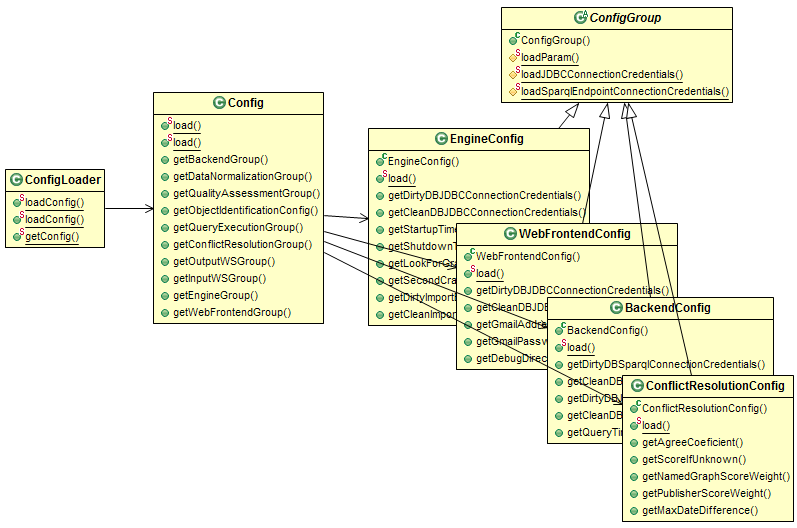
\includegraphics[width=0.8\textwidth]{images/dia-core-config.png}
    \caption{Diagram of (selected) configuration classes}
	\label{fig:configurationClasses}
\end{figure}

Configuration for each component is in classes called \code{XXXConfig} inheriting from \code{ConfigGroup}. Each instance of \code{ConfigGroup} loads configuration relevant only for that component so as to minimize dependencies. Configurations for all components are grouped in \code{Config} class accessible from \code{ConfigLoader}.

\section{Database Access}
Classes \code{JDBCConnectionCredentials} and \code{SparqlEndpointConnectionCredentials} are containers for information necessary for connecting to the database.

\FE uses its own database access layer using Spring templates. The rest of \odcs should use classes \code{VirtuosoConnectionWrapper} and \code{WrappedResultSet}. These two classes provide methods for both querying and updating the relational database and working with SPARQL. They also provide methods for conversion of Virtuoso SQL types to Java types, working with transactions etc. Note that SPARQL update operations should be executed with log level set to AUTOCOMMIT (default).

Use of \code{VirtuosoConnectionWrapper} is also recommended for implementation of custom transformers. An example of how it can be used is in  \lstlistingname~\ref{lst:virtuosoConnectionWrapper}.

\begin{lstlisting}[caption={Example of programmatic access to Virtuoso database from a transformer},label=lst:virtuosoConnectionWrapper]

  @Override
  public void transformGraph(TransformedGraph inputGraph, TransformationContext context)
      throws TransformerException {
    VirtuosoConnectionWrapper connection = null;
    WrappedResultSet resultSet = null;
    try {
      connection = VirtuosoConnectionWrapper.createConnection(
          context.getDirtyDatabaseCredentials());

      String query1 = "SPARQL SELECT ?s WHERE {?s ?p ?o}";
      resultSet = connection.executeSelect(query1)
      while (resultSet.next()) {
        String s = resultSet.getString("s");
      }

      String query2 = "SPARQL INSERT INTO <a> { <b> <c> <d> }";
      connection.execute(query2);
    } catch (DatabaseException e) {
      throw new TransformerException(e);
    } catch (SQLException e) {
      throw new TransformerException(e);
    } finally {
      if (resultSet != null) { resultSet.closeQuietly(); }
      if (connection != null) { connection.closeQuietly(); }
    }
  }
\end{lstlisting}

\section{Data Import}
When importing data to Virtuoso, one should use the \code{GraphLoader}  class or methods in \code{VirtuosoConnectionWrapper}. These make Virtuoso import the data itself. Other methods, such as using the Jena library may fail when used with too large data. Note that when importing from a file, it must be in directory listed in \code{DirsAllowed} directive of Virtuoso. See also \code{engine.clean\_import\_export\_dir} configuration option.

%%%%%%%%%%%%%%%%%%%%%%%%%%%%%%%%%%%%%%%%%%%%%%%%%%%%%%%%%%%%%%%%%%%%%%%%%%%%%%
\chapter{Engine}
\section{Purpose}
Engine runs the whole server part. This is the component that actually processes the RDF data. It also starts Input and Output Webservices and thus provides the outer interface for accepting data and querying over data.





\section{Implementation}
Class \code{Engine} contains the \code{main()} method which represents the entry point of the application. It checks the environment, loads and validates configuration and starts the services that Engine consists of. Thereafter, Engine periodically updates its state in the database (for monitoring from \FE) and waits for shutdown (using the standard JVM shutdown hook).

There are timeouts for service initialization and shut down. When the timeout is exceeded, the service is finished forcibly and Engine stops.

\subsection{Services}
Engine consists of three independent services: 
\code{InputWSService}, \code{OutputWSService}, and \code{PipelineService} for Input Webservice, Output Webservice and pipeline processing, respectively. Services inherit from a common base class \code{Service}. Services are initialized and started as soon as Engine is started and can be asynchronously shut down when Engine is being shut down. Services have their own state and inform \code{Engine} about its changes. 

Engine is implemented as a multithreaded server. Multiple requests for both Input and Output Webservice can be handled at the same time. The data processing part processes named graphs sequentially, one at a time. Engine is implemented so that extending to parallel data procesing should be simple, however. 

\subsection{Transactional Processing}
\label{sec:transactionalProcessing}
Data processing in \odcs is done by running a pipeline of transformers on the processed set of named graphs. Running a pipeline is a long-lasting operation on potentionally large data. Databases, including Virtuoso, usually process such operations in a non-transactional way. Engine, however, ensures a transactional character of running a pipeline. 

As long as used transformers adhere to the contract specified in Section \ref{sec:transformerContract}, pipelines have all ACID properties. In addition, an increased attention was given to robustness of Engine to errors. The foundation of this robustness is in implementation that ensures that Engine can be shut down at any time without permanent loss of data integrity. These features were accomplished in the following way:
\begin{enumerate}
  \item RDF data processing is divided into a sequence of operations that move from one consistent state to another consistent state.
  \item All changes of state data at the beginning and end of each operation are executed strictly in a context of single transaction in the relational database.
  \item In case of an error during an operation, the operation can be always either rolled back or finished.
  \item Data processing is executed in the isolated dirty database instance so that inconsistent states of data being processed are invisible to the outside. 
  \item \label{itm:enginePrefix} Since moving data from the dirty database instance to the clean database instance cannot be executed in a transaction, the named graphs inserted to the clean database are made invisible to \QE by adding a special prefix to their names. \QE ignores all graphs with this prefix. After the import is complete, the named graphs are renamed and made visible for queries. If the new data in the clean database replace older data after re-running a pipeline on them, the old data would be made invisible at the same time by adding the special prefix to them and deleted afterwards.
\end{enumerate}

Several other mechanisms for transactional processing provided by Virtuoso were examined during development. They proved very limiting and often even caused the database instance to crash, however. Transactions for RDF data in Virtuoso were rejected for this reason and transactional properties are ensured by the mechanism presented above.    

All services are also resilient to a loss of database connection. Engine doesn't need to restart when the connection is regained again. Input Webservice and pipeline processing require connection to both database instances, Output Webservice needs only the clean database instance.

\subsection{Database Access}
Engine uses class \code{DbOdcsContext} extending \code{DbContext}
which wraps \code{VirtuosoConnectionWrapper} and provides transactional processing of relational data. 
Class \code{SQL} contains all SQL queries used by \code{DbOdcsContext}. 

Note that relational database (in the clean database instance) is also the only means of communication with \FE. Settings for Engine managed in \FE are written to relational database from where Engine loads it and vice versa -- Engine updates its status and state of graphs processing in the relational database from where \FE can load it.

\section{Input Webservice}
\subsection{Purpose and Features}
Input Webservice is a multithreaded SOAP webservice that accepts new data and queues them for data processing by a pipeline. It is implemented with a streaming SOAP message processing so that memory usage is minimized and even large data can be accepted. Input Webservice also supports secure communication over HTTPS. 

The counterpart of Input Webservice on the client side is \code{odcs-inputclient} library which is provided to data producers for convenience. Shared parts of Input Webservice and \code{odcs-inputclient} are in library \code{odcs-comlib}. \code{odcs-comlib} is implemented with minimum memory requirements compared to the standard jax-ws implementation. Received data are evaluated as soon as they are received and errors are reported to the client immediately (unlike jax-ws). Streaming processing of the SOAP message is implemented using \code{javax.xml.parsers.SAXParser} supplemented by SOAP 1.1 envelope schema validation in \code{odcs-comlib}. 

WSDL and XSD schema of the SOAP service are parts of Input Webservice as embedded resources and dynamically served according to the HTTP request.

When Input Webservice is started, it starts a HTTP server listening on a given port and then tries to run recovery. If there are any unfinished requests from the previous run, then their records in the database and data files are deleted. HTTP 503 -- Service unavailable response is given until recovery is finished.

Shutdown of the service stops all pending requests and the HTTP server.

\subsection{Implementation}
The implementation is in classes \code{SoapMethodInsertExecutor} extending \code{SoapMethodExecutor} in a way similar to the standard \code{DefaultHandler} for \code{SAXParser}. \code{SoapMethodExecutor} is part of \code{odcs-comlib} and filters out parts of the message that belong to the SOAP protocol. The main execution part of message processing is in the \code{InsertExecutor} class which subsequently takes input parameters and saves received data to the filesystem as files with suffix \code{-d.ttl} or \code{-d.rdf} for the payload data, suffix \code{-m.ttl} or \code{-m.rdf} for metadata and \code{-pvm.ttl} or \code{-pvm.rdf} for provenance metadata, depending on the serialization format (Turtle or RDF/XML). In case of success, it signalizes that a new named graph was accepted to pipeline service which will eventually run a transformer pipeline on the new data.

If updating the state of processing in the relational database fails, Input Webservice retries with in an interval defined in global configuration. If the process of receiving data fails in other cases, \code{InsertExecutor} throws an \code{InsertExecutorException} exception which can assemble a \code{InsertException} SOAP message for the client. These messages are sent in \code{InputWSHttpServer} together with other errors in the SOAP protocol. Created files are deleted on error and so are records of the import in the relational database. 


\section{Pipeline Service}
\subsection{Purpose}
Pipeline Service is responsible for processing of data which are marked to be processed or deleted. Data processing is realized by transformers that are applied to a set of related named graphs in a pipeline. Pipelines work exclusively on data in the dirty database instance and pipeline service is responsible to move the data to the clean database when a pipeline finishes successfully.

Data to be processed are either new named graphs stored through Input Webservice, or data that were marked for deletion  or for processing in \FE. The last case occurs when a user chooses to re-run a~pipeline on data already stored in the clean database. Copy of this data is created in the dirty database where it is processed by the pipeline. After that, the processed version of data replaces the original in the clean database.

\subsection{Graph States}
Every named graph inserted through Input Webservice has a record in relational table \code{DB.ODCLEANSTORE.EN\_INPUT\_GRAPHS} with an associated state, among other things. The states can be:

\begin{description}[style=nextline,font=\ttfamily]
  \item[IMPORTING] The named graph is being imported through Input Webservice.
  \item[QUEUED\_FOR\_DELETE] The named graph is queued for deletion. When a graph is deleted, all related graphs in both database instances are deleted. Related temporary files are deleted as well.
  \item[QUEUED\_URGENT] Reserved for future use.
  \item[QUEUED] Named graph is queued to be processed by its respective pipeline.
  \item[PROCESSING] Named graph is  being processed in a pipeline. That means the graph is loaded from temporary Input Webservice files or the clean database, and pipeline transformers are applied to it. All settings for the pipeline including the plan of transformers to execute and their assigned rule groups are loaded only when the graph transitions to this state so that their consistency during the pipeline processing is ensured.
  \item[PROCESSED] Transformers were successfully applied to the named graph and the data are being moved to the clean database into named graphs whose name starts with a special prefix hiding them from \QE (see point \ref{itm:enginePrefix} in Section \ref{sec:transactionalProcessing}). Let us call this prefix the \term{temporary prefix}.
  \item[PROPAGATED] The processed named graphs were all moved to the clean database. If there was an old version of the data, the old named graphs are prefixed with the temporary prefix.
  \item[OLDGRAPHSPREFIXED] The temporary prefix is removed from the processed graphs and the possible old versions of named graphs, now prefixed with the temporary prefix, are removed.
  \item[NEWGRAPHSPREPARED] Related graphs in the dirty database are deleted.
  \item[FINISHED] The processing of the named graphs was successfully finished and the data are stored in the clean database.
  \item[DELETING] The named graphs are being deleted in the clean and/or dirty database instance. Possible temporary files stored by Input Webservice will be also deleted.
  \item[DELETED] The named graph was successfully deleted.
  \item[WRONG] An error occurred during the named graph processing.
  \item[DIRTY] If an error occurs while the named graph is in state \code{PROCESSING} or \code{PROCESSED}, the graph is first marked as \code{DIRTY} and Engine cleans up unfinished work and only after that the graph is moved to state \code{WRONG}.
\end{description}

\subsection{Implementation}
Data processing in Engine is driven by settings in the relational database which are managed from \FE. 

Engine logs its activity to a log file called odcs.engine.log in the working directory of Engine. In addition, there is a log file for each transformer instance where the respective transformer logs its activity. These transformer instance logs are in the working directory of the respective transformer.

When shutdown is called on the pipeline processing service then if there is a running transformer, its \code{shutdown()} method is called. Engine waits until the current operation is finished or the given timeout is exceeded and the finishes the pipeline processing service. 

Running a pipeline is transactionally safe, as explained in Section \ref{sec:transactionalProcessing}.  If an error is caused by Engine (e.g. when it is shut down forcibly), the pending operations will be finished eventually. When an error occurs and a graph is in \code{PROPAGATED}, \code{OLDGRAPHSPREFIXED} or \code{NEWGRAPHSPREPARED}, the pipeline service continues in a forward way on recovery; other temporary states are rolled back. If an error is caused by a transformer, then the named graph is moved to state \code{WRONG} and it is up to the user to decide what to do next with the graph. An overview of failed graphs is in \FE. The reason why the transformer failed can be fixed and the pipeline re-run on the graph, or the graph may be queud for deletion.

If an error is caused by unavailability of a Virtuoso database, Engine detects it and pending processing is retried when Engine is started again.

Classes that cover implementation of pipeline service are \code{PipelineService}, which handles processing of named graphs in different states, \code{PipelineGraphManipulator} for manipulation with named graphs (e.g. moving between database instances) and \code{PipelineGraphStatus} for working with state data (e.g. loaded transformer instances for the processing pipelines). \code{PipelineGraphTransformerExecutor} called from \code{PipelineService} is responsible for executing transformers on named graphs and \code{TransformationContext} and \code{TransformationGraph} are implementations of context objects passed to transformers.


\section{Output Webservice}
\subsection{Purpose}
Output Webservice is a RESTful webservices for queries over data in the clean database. More details about types of queries and request format are described in \refusermanual.

\subsection{Implementation}
Output Webservice is built on top of the Restlet library. \code{OutputWSService} started by Engine registers a Restlet application implemented by class \code{Root} which sets up URI routes and handlers for each type of query.

Each type of query is handled by a class inheriting from \code{QueryExecutorResourceBase} which in turn implements Restlet \code{ServerResource}. This base class loads necessary configuration and handles requests (methods annotated with Restlet \code{@Get} and \code{@Post} annotations) -- parses request parameters (as described in \refusermanual), delegates the execution to the abstract \code{execute()} method implemented in child classes and handles returning of a proper response in case of an error.

\begin{figure}[htb]
    \centering
    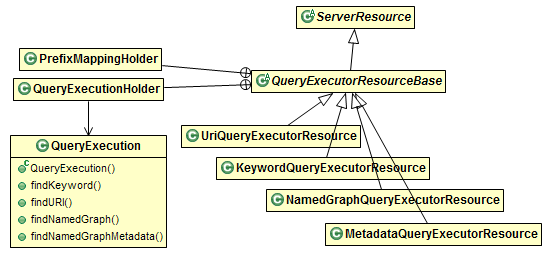
\includegraphics[width=0.7\textwidth]{images/dia-outputws-resources.png}
    \caption{Diagram of selected Output Webservice classes}
	\label{fig:outputwsResources}
\end{figure}


Classes implementing the actual execution of the query are \code{UriQueryExecutorResource}, \code{KeywordQueryExecutorResource}, \code{NamedGraphQueryExecutorResource} and \linebreak[4] \code{MetadataQueryExecutorResource}. They redefine the abstract \code{execute()} method where query-specific parameters are parsed and the execution is delegated to the Query Execution component. Instance of the \code{QueryExecution} class is shared between requests in order to utilize caching implemented in Query Execution. Finally, the result of the query is formatted and sent to the user.

\subsection{Output Formatters}
Query results returned from Query Execution are formatted using the format requested by the user. Formatting is done by classes implementing \code{QueryResultFormatter}.

The default formatter is \code{HTMLFormatter} which outputs results in HTML. \code{RDFXMLFormatter} and \code{TriGFormatter} inherit from \code{RDFFormatter} and output results in RDF/XML and TriG, respectively. \code{DebugFormatter} formats result for output to console and is not accessible for users.

\begin{figure}[htb]
    \centering
    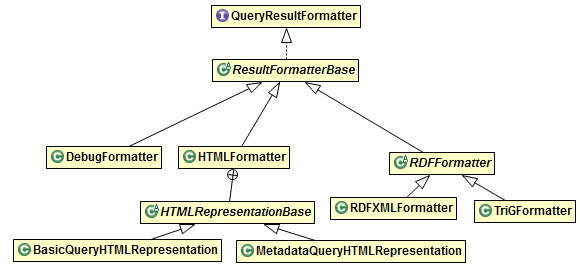
\includegraphics[width=0.8\textwidth]{images/dia-outputws-formatters.png}
    \caption{Diagram of output formatters hierarchy}
	\label{fig:outputwsFormatters}
\end{figure}

\subsection{Extending}
In order to add a new type of query to Output Webservice, the following steps should be taken:

\begin{enumerate}
	\item Implement a new \code{ServerResource} executing the query, preferably inheriting from \linebreak[4] \code{QueryExecutorResourceBase}. Typically, the actual query will be delegated to the Query Execution component -- see Section \ref{sec:qeExtending}.
	\item Register the new \code{ServerResource} in method \code{Root\#createInboundRoot()}.
\end{enumerate}


%%%%%%%%%%%%%%%%%%%%%%%%%%%%%%%%%%%%%%%%%%%%%%%%%%%%%%%%%%%%%%%%%%%%%%%%%%%%%%
\chapter{Query Execution}
\label{sec:QE}

\section{Purpose}
The purpose of \QE is to retrieve result for a query (asked through Input Webservice), resolve conflicts using the \CR and return result.

Triples that \QE retrieves are:
\begin{enumerate}
	\item \label{item:queryTriples} Triples relevant for the query (e.g. containing the given URI).
	\item Triples with metadata about named graphs containing triples from (\ref{item:queryTriples}).
	\item Triples containing human-readable labels for URI resources occuring in triples from (\ref{item:queryTriples}).
\end{enumerate}
A special case is the metadata query which retrieves only named graph metadata.

Because the result of conflict resolution depends on the data it is given, \QE and \CR are not independent but rather \QE extracts exactly the data that \CR needs and calls it directly.

\section{Interface}
The public interface of the \QE component is represented by class \code{QueryExecution}.

 This class exposes methods for executing all kinds of supported queries and returns result as an instance of \code{MetadataQueryResult} (wraps collection of provenance metadata triples and other metadata) or \code{BasicQueryResult} (wraps collection of \code{CRQuad}s returned from \CR plus metadata). The query can be further parametrized by passing \code{QueryConstraintSpec} and \code{AggregationSpec} affecting the retrieved data and the conflict resolution process, respectively.

 \code{QueryExecution} is thread-safe and its instance should be kept between requests in order to effectively utilize caching.

\section{Implementation}
The actual implementation is in classes inheriting from \code{QueryExecutorBase}, each implementing one type of query: \code{URIQueryExecutor}, \code{KeywordQueryExecutor}, \code{NamedGraphQueryExecutor} and \code{MetadataQueryExecutor}. These classes are called internally from the \code{QueryExecution} class. Implementing classes are in Java package \code{cz.cuni.mff.odcleanstore.queryexecution}.

\begin{figure}[htb]
    \centering
    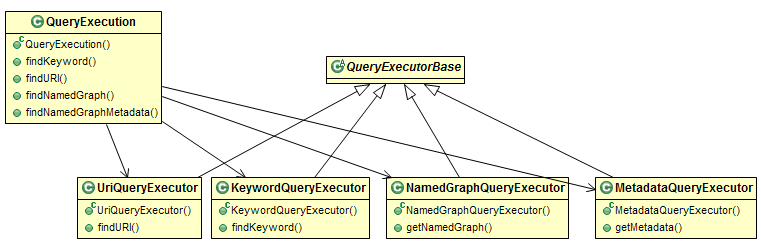
\includegraphics[width=0.8\textwidth]{images/dia-qe.png}
    \caption{Diagram of main Query Execution classes}
	\label{fig:qeClasses}
\end{figure}

For each query, the following steps are executed: input is validated, result quads retrieved from the database, metadata and labels are retrieved from the database and conflict resolution is applied to the result.

To improve performance, values that are used for each query but rarely changed are cached. Cached values are: default aggregation settings, prefix mappings and label properties.

\section{Extending}
\label{sec:qeExtending}
In order to implement a new type of query, the following steps should be taken:

\begin{enumerate}
	\item Create a class implementating the new query, preferably inheriting from \code{QueryExecutorBase}.
	\item Extend \code{QueryExecution} class with method for executing the query.
	\item Extend Input Webservice to provide access to the new query for users.
\end{enumerate}

\section{Database}
\QE retrieves RDF data from the clean database instance. Because Virtuoso doesn't fully support transactions with RDF data, the clean database may contain incomplete data partially inserted by Engine. In order to filter such data from the result, \QE ignores all named graphs whose URI starts with an agreed prefix\footnote{\code{http://opendata.cz/infrastructure/odcleanstore/internal/hiddenGraph/}} given by Engine to such named graphs.

In addition, \QE loads settings from the following tables in relational database (see Appendix \ref{chap:reldb}):

\begin{itemize}
	\item \dbodcs{qe\_label\_properties}
	\item \dbodcs{cr\_properties} 
	\item \dbodcs{cr\_settings} 
	\item and tables referenced from tables above
\end{itemize}

%%%%%%%%%%%%%%%%%%%%%%%%%%%%%%%%%%%%%%%%%%%%%%%%%%%%%%%%%%%%%%%%%%%%%%%%%%%%%%
\chapter{Conflict Resolution}
\label{sec:CR}

\section{Purpose}
Data stored in \odcs may come from multiple sources and conflicting statements may emerge. For example, data about a city stored in \odcs may state multiple different values for its population. The purpose of \CR is to resolve such conflicts according to default or user-defined policies (e.g. show the latest, average or all values for the population). In addition, it computes an estimate of \aggrq of each RDF triple in the resulting data and provides provenance tracking, 	i.e. provides URIs and metadata of named graphs from which the resulting value was selected or calculated from. Finally, \CR can filter out old versions of data for which a newer version was inserted.

\todo{}

\section{Interface}
Interface of the \CR component is represented by Java interface \code{ConflictResolver}. It contains a single operation:
\begin{verbatim}
      Collection<CRQuad> resolveConflicts(Collection<Quad> quads)
          throws ConflictResolutionException;
\end{verbatim}
\CR accepts a collection of quads (RDF triple + named graph) and returns a collection of \code{CRQuad}s (quad + \aggrq + source named graphs).

An instance of \code{ConflictResolver} can be obtained from factory class \code{ConflictResolverFactory}. Constructor of this class takes query-independent settings and its \code{createResolver()} methods takes query-dependent settings (named graph metadata, sameAs links, aggregation settings, preferred URIs) and returns a new instance of \code{ConflictResolver} for these settings. The~signatures of the constructor and the \code{createResolver()} method are in \lstlistingname~\ref{lst:crFactory}.

\begin{lstlisting}[caption={\code{ConflictResolverFactory} interface},label=lst:crFactory]
      public ConflictResolverFactory(
          String resultGraphPrefix,
          ConflictResolutionConfig globalConfig,
          AggregationSpec defaultAggregationSpec)

      public ConflictResolver createResolver(
            AggregationSpec aggregationSpec,
            NamedGraphMetadataMap metadata,
            Iterator<Triple> sameAsLinks,
            Set<String> preferredURIs)
\end{lstlisting}

\section{Implementation}
The actual implementation of the \code{ConflictResolver} interface is in class \code{ConflictResolverImpl}. Its constructor requires two parameters -- one of type \code{ConflictResolverSpec} contains all settings for conflict resolution and one of type \code{ConflictResolutionConfig} is a container for global settings (configurable in the \odcs configuration file). \code{ConflictResolverSpec} contains default and per-property aggregation methods to be used, metadata of relevant named graphs including \QA scores, additional \code{owl:sameAs} links to consider and other technical settings.

Implementation of the \code{resolveConflicts()} methods does the following:

\begin{enumerate}
	\item \code{owl:sameAs} links are used to find resources representing the same entity. The implementation is in class \code{URIMappingImpl} which uses the DFU (Disjoint Find and Union) data structure with path compression to find weakly connected components of the \code{owl:sameAs} links graph.
	\item URI resources in input quads are translated so that a single URI is used for every resource representing the same entity using mapping created in the previous step.
	\item The resulting quads are sorted and grouped to clusters of (potentially) \term{conflicting quads}, i.e. those sharing the same subject and predicate. Implemented in \code{ResolveQuadCollection}.
	\item \CR iterates over groups of conflicting quads and applies the actual conflict resolution procedure.
		\begin{enumerate}
			\item The next group of conflicting quads is retrieved. All such quads have the same value in place of the subject and predicate.
			\item If there are Identical triples which come from named graphs where one named graph is an update of the other named graphs, the old versions are removed (see Section \ref{sec:latestUpdateMarker} for definition of an update).
			\item An aggregation method is chosen based on the predicate of quads in the current group and conflict resolution settings.
			\item \label{item:crAggr}
				The aggregation method is applied to the current group of conflicting quads. The output is a collection of \code{CRQuad}s and it is added to the result.
		\end{enumerate}
	\item The resulting \code{CRQuad}s are returned.
\end{enumerate}

We call steps 1-3 \term{implicit conflict resolution} and it doesn't depend on the given aggregation settings. It prepares input data for step 4 so that result quads and \aggrq can be computed independently on chosen resource URIs. Its time complexity is $\mathcal{O}(S \log S + N \log N)$ where $S$ is the number of \code{owl:sameAs} links and $N$ number of input quads. Step 4 is applied to sets of conflicting quads having the same subject and predicate so the context of aggregation is given mainly by quad objects.

\subsection{Aggregation Methods}
\CR accepts an argument of type \code{ConflictResolverSpec} which specifies which agregation method should be used for which predicate, among other things. This is set either by the user as a parameter of Output Webservice or a default setting in \odcs is used.
The selected aggregation method determines how conflicts are resolved and \aggrq of the result is computed in step \ref{item:crAggr} of the conflict resolution algorithm.

An aggregation method is represented by Java interface \code{AggregationMethod} with the following method:

\begin{verbatim}
      Collection<CRQuad> aggregate(
          Collection<Quad> conflictingQuads, 
          NamedGraphMetadataMap metadata);
\end{verbatim}

Objects implementing \code{AggregationMethod} are created by \code{AggregationMethodFactory}. Classes implementing an aggregation method inherit from \code{AggregationMethodBase} and their hierarchy is depicted on \figurename~\ref{fig:crAggregations}.

\begin{figure}[htb]
    \centering
    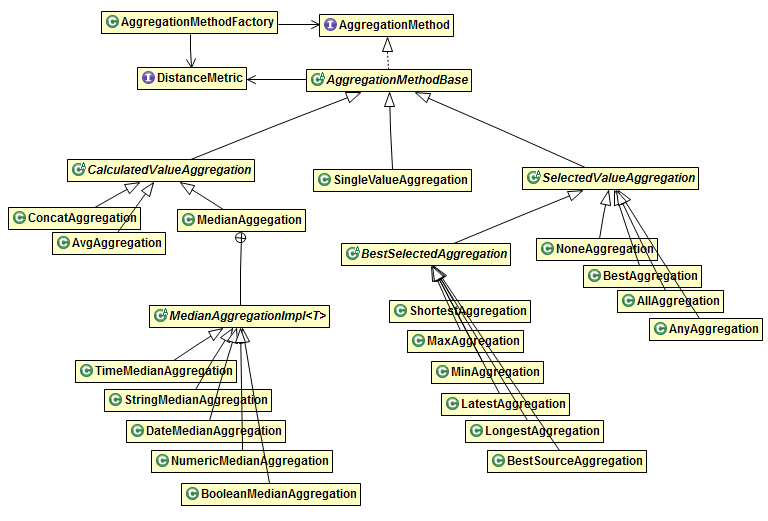
\includegraphics[width=\textwidth]{images/dia-cr-aggregations.png}
    \caption{Implementation classes of aggregation methods}
	\label{fig:crAggregations}
\end{figure}

There are two basic types of aggregations. First type called \term{selected aggregations} selects one or more quads from input quads while the result of the second type called \term{calculated aggregation} returns values computed from all the input quads (e.g. average). The common functionality of these two types is in abstract classes \code{CalculatedValueAggregation} and \code{SelectedValueAggregation}.

A special type of selected aggregation is \code{BestSelectedAggregation} which selects a single best quad based on a metric given as an instance of \code{AggregationComparator} (\figurename~\ref{fig:crComparators}).

As an optimization, if there is only a single quad in a group of conflicting quads, a special optimized \code{SingleValueAggregation} aggregation can be used because all aggregation methods should return the same result in this case.

If the selected aggregation method cannot be applied to a value (e.g. average of a string literal), the behavior depends on the given aggregaiton error strategy - the value may be either discarded, or included in the result without aggregation applied.

More details about each aggregation method and their time complexity can be found in javadoc of the respective classes.

\begin{figure}[htb]
    \centering
    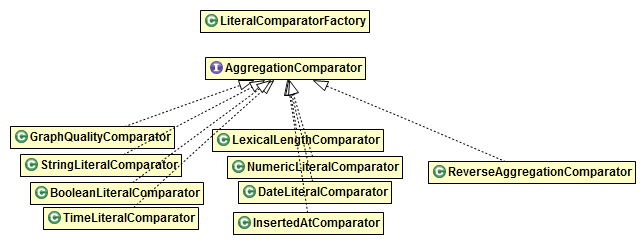
\includegraphics[width=\textwidth]{images/dia-cr-comparators.png}
    \caption{Comparators for \code{BestSelectedAggregation}}
	\label{fig:crComparators}
\end{figure}
	
\subsection{Quality and Provenance Calculation}
The aggregation methods described in the previous section solve conflicts by calculating or selecting values in place of the object of a quad (e.g. choose the quad with the highest \QA score, the latest insertion date, maximum value in place of the object, or calculate the average of all values in place of the object). In addition, they add provenance and quality information.

The provenance information consists of a list of named graphs, let us denote them \term{source named graphs}, from which the result was selected or calculated from. For calculated aggregations, these are named graphs of all aggregated quads, for selected aggregations these are named graphs containing the quad(s) selected to the result.

The \aggrq estimate is done for each result quad and is based on several factors based on real-world scenarios: quality scores of the source named graphs, number of graphs that agree on a value and the difference between a value and other (conflicting) values.

\subsubsection{Notation}
An aggregation method works on quads having the same subject and predicate and they may only differ in the object and the named graph. Let $n$ be the number of aggregated quads (in a single group of conflicting quads). Let $o_i$ be the value in place of object and $g_i$ the named graph of $i$-th quad.

Let $s_{ng}(g)$ denote the \QA score of a named graph $g$ and $s_p(g)$ the average score of publishers of the named graphs. Both these values are given in named graph metadata as input of conflict resolution (they are computed in advance by \QA and Quality Aggregator transformers, respectively). $s(g)$  denotes the total score of a named graph based on $s_{ng}(g)$ and $s_p(g)$ (see Section~\ref{sec:qualityCalculation}).

Let $agree(v)$ denote the set of named graphs that agree on the value $v$, i.e. $$agree(v) = \left\{g_i~|~v_i=v\right\}.$$

Finally let $q(v)$ denote the \aggrq of a result quad that has value $v$ as its object.

\subsubsection{Constraints on Quality Calculation}
The algorithm calculating \aggrq was designed so that several constraints hold:
\begin{itemize}
	\item If $n= 1$, then $q(v_1) = s(g_1)$.
	\item If there is a named graph $g$ asserting a non-conflicting value $v$, the quality (based just on the value $v$) should be at least $s(g)$.
	\item $q(v)$ is increasing with \QA scores of source named graphs of quads having $v$ as object.
	\item $q(v)$ is decreasing with increasing difference from other object values in input quads, taking their \QA scores into consideration (higher \QA score means higher weight of the value).
	\item If multiple source named graphs agree on the same value $v$, then $q(v)$ is increased.
	\item If $k$ sources with \QA scores equal to 1 (highest score) claim a value completely different from value $v$, then quality of $v$ should be decreased approximately $k$ times. If the sources have lower \QA scores, the decrease should be lower.
\end{itemize}

\subsubsection{Quality Calculation}
\label{sec:qualityCalculation}
Aggregate quality $q(v)$ is calculated in the following steps:
\begin{enumerate}
	\item A total \QA score $s(g)$ for each source named graph is determined. It is calculated as
		$$s(g) = \alpha s_{ng}(g) + (1-\alpha) s_p(g),$$

		where $\alpha\in[0,1]$ is a configurable parameter.
	\item Quality based on source named graphs is calculated. For each quad object value $v$, we compute quality based on source named graphs, let us denote it $q_1(v)$.

		$$q_1(v) = \begin{cases}
				\mathrm{avg} \left\{s(g)~|~g\in \left\{g_1,\ldots,g_n\right\}	\right\} & \mbox{calculated aggregations} \\
				\max \left\{s(g)~|~g\in agree(v)\right\} & \mbox{selected aggregations}
			\end{cases} $$
	\item Next, the differences between conflicting values are taken into consideration. We use a metric $d:U\times U\rightarrow[0,1]$ satisfying $d(v,v)=0$ for this purpose.

		We use $d(x,y)=|(x-y) / \mathrm{avg}(x,y)|$ in case of numeric literals, normalized Levenshtein distance in case of string literals, difference divided by a configurable maximum value in case of dates and $d(x,y)=1$, where $x\neq y$, for URI resources, blank nodes and nodes of incompatible types.

		Whether decreasing the aggregate quality based on conflicting values is the right solution depends on context, however. Predicate \code{rdf:type} often has multiple valid values which are not in fact conflicting. Therefore, whether to decrease score based on conflicts is set by the \term{multivalue} setting for the current predicate.
		
		If multivalue is false and there are conflicting values different from $v$, the  quality of $v$ is reduced increasingly with the value of metric $d$ and the score of the source of the conflicting value:

		$$q_2(v) = \begin{cases}
				q_1(v) \cdot \left(1- \frac{\sum_{i=1}^{n}s(g_i)d(v,v_i)}{\sum_{i=1}^ns(g_i)}\right) & \mbox{multivalue is false for the current property}\\
				q_1(v) & \mbox{multivalue is true for the current property} 
			\end{cases}
		$$
		
	\item Aggregate quality should be increased if multiple values agree on the same value.
		$$q_3(v) = q_2(v)+(1-q_2(v))\cdot \min \left(\frac{-q_1(v)+\sum_{g\in agree(v)} s(g)}{C}, 1\right),$$
		where $C\in\mathbb{N}$ is a configurable constant.
	\item Each aggregation method may adjust the general algorithm. In case of the CONCAT aggregation, computing $q_2$ and $q_3$ doesn't make sense and $q(v)=q_1(v)$ is returned. AVG and MEDIAN aggregations return $q(v)=q_2(v)$, and finally $q(v)=q_3(v)$ is returned for other aggregations.
\end{enumerate}

\subsubsection{Time Complexity}
\label{aggrTimeComplexity}
The time complexity of the \aggrq computation for a fixed value $v$ is $\mathcal{O}(n\cdot D)$, where $D$ is the complexity of the distance metric evaluation. This gives us the overall complexity of $\mathcal{O} (n^2 \cdot D)$ for ALL and BEST aggregations, $\mathcal{O}(n \log n + n \cdot D$ for MEDIAN and $\mathcal{O}(n\cdot D)$ for others.

\section{Time Complexity}
Let $N$ be the total number of input quads of the conflict resolution process, $S$ number of \code{owl:sameAs} links, $G$ number of named graphs for which we have metadata given. Let $CQ=\left\{cq_1, cq_2, \ldots, cq_K\right\}$ be the set of groups of conflicting quads and $n_i=|cq_i|$ be the size of $i$-th group of conflicting quads. $D$ is the complexity of distance metric evaluation.

The complexity of implicit conflict resolution algorithm is $\mathcal{O}(N \log N + S\log S)$. Grouping the quads into clusters of conflicting quads requires sorting in $\mathcal{O}(N \log N)$, assuming comparison of two RDF nodes is in constant time. Filtering of old versions is implemented in $\mathcal{O}(n_i \log n_i \log G)$ (\code{NamedGraphMetadataMap} is implemented using a \code{TreeMap}, could be improved to $\mathcal{O}(n_i\log n_i)$ with a \code{HashMap}). Finally an aggregation method is applied with complexity given in Section \ref{aggrTimeComplexity}.

To sum up, the total time complexity is:
\begin{itemize}
	\item In case of ALL and BEST aggregation:
		$$ \mathcal{O}\left(N \log N + S\log S + \sum_{i=1}^K \left(n_i \log n_i \log G + n_i^2 D\right)\right)$$
	\item For aggregations other than ALL, BEST and MEDIAN:
	$$ \mathcal{O}\left(N \log N + S\log S + \sum_{i=1}^K \left(n_i \log n_i \log G + n_i D\right)\right)$$
\end{itemize}

In the worst case when $K = 1$ and $G = N$ ($G\leq N$ because at most $N$ named graphs can be among input quads and \CR gets in fact metadata only for these named graphs), this gives us

\begin{itemize}
	\item In case of ALL and BEST aggregation:
		$$ \mathcal{O}\left(N^2 D+S\log S\right)$$
	\item For aggregations other than ALL, BEST and MEDIAN:
	$$ \mathcal{O}\left( N \log^2 N + ND+S\log S \right)$$
\end{itemize}

Distance metric is evaluated in linear time for strings (modified Levenshtein distance) and in constant time for other cases.

\section{Extending}
In order to add a new aggregation method, the following steps should be taken:
\begin{enumerate}
	\item Implement the aggregation in a class implementing the \code{AggregationMethod} interface.
	\item Create a constant representing this aggregation method in enum \code{EnumAggregationType}.
	\item Extend \code{AggregationMethodFactory} to create an instance of the new aggregation.
\end{enumerate}

If a new distance metric for a specific type of literal is to be added, this should be done in the \code{DistanceMetricImpl} class.


%%%%%%%%%%%%%%%%%%%%%%%%%%%%%%%%%%%%%%%%%%%%%%%%%%%%%%%%%%%%%%%%%%%%%%%%%%%%%%
\chapter{Transformers -- Introduction}
In this section, by a transformer we mean a Java class implementing the \code{Transformer} interface shown in \lstlistingname~\ref{lst:transformer} (and other related classes used for implementation).

\begin{lstlisting}[caption={Transformer interface},label=lst:transformer]
  package cz.cuni.mff.odcleanstore.transformer;
  public interface Transformer {
    void transformGraph(TransformedGraph inputGraph, TransformationContext context)
         throws TransformerException;

    void shutdown() throws TransformerException;
}
\end{lstlisting}

The purpose of a transformer is to somehow process data. The data are not passed in memory, but rather stored in the (dirty) database instance and only the URI of the named graph to be processed and connection credentials for accessing the database are given to the transformer. This should minimize the need of complicated interfaces for data passing, make it easier to work with large data, let the transformer choose its own method of accessing the database and give it the full power of SPARQL/SPARUL (as implemented in Virtuoso).

The actual data processing should be implemented in the \code{transformGraph()} method. All required information is passed in its arguments, one with information about the processed graph and one about the environment -- see \lstlistingname{}s~\ref{lst:transformedGraph} and \ref{lst:transformationContext}.

The \code{shutdown} method is called when Engine shuts down and can be used e.g. to release acquired resources.

\begin{lstlisting}[caption={TransformedGraph interface},label=lst:transformedGraph]
  package cz.cuni.mff.odcleanstore.transformer;
  import java.util.Collection;

  public interface TransformedGraph {
    String getGraphName();
    String getGraphId();
    String getMetadataGraphName();
    String getProvenanceMetadataGraphName();
    Collection<String> getAttachedGraphNames();
    void addAttachedGraph(String attachedGraphName) throws TransformedGraphException;
    void deleteGraph() throws TransformedGraphException;
    boolean isDeleted();
  }
\end{lstlisting}

\begin{lstlisting}[caption={TransformationContext interface},label=lst:transformationContext]
  package cz.cuni.mff.odcleanstore.transformer;
  import java.io.File;
  import cz.cuni.mff.odcleanstore.connection.JDBCConnectionCredentials;

  public interface TransformationContext {
    JDBCConnectionCredentials getDirtyDatabaseCredentials();
    JDBCConnectionCredentials getCleanDatabaseCredentials();
    String getTransformerConfiguration();
    File getTransformerDirectory();
    EnumTransformationType getTransformationType(); /* NEW or EXISTING */
  }
\end{lstlisting}

\section{Transformer Instance Configuration}
\label{sec:transformerInstConfig}
Each instance of a transformer in a pipeline may have its own configuration (for explanation of the difference between \term{transformer} and \term{transformer instance}, see Section \ref{sec:dataProcessing}). From the point of view of a transformer, it is a plain string which can be obtained by calling the \code{getTransformerConfiguration()} method.

This configuration string can be edited in \FE. The transformer may use the value in any way it needs, e.g. it may contain XML configuration, the recommended practice is to use the Java \code{Properties} file format, however. This format is used by transformers included by default in \odcs unless stated otherwise.

Instances of important transformers (\QA, \DN, \OI) can be also configured by assigning rule groups to them in \FE.

\section{Contract between Engine and Transformers}
\label{sec:transformerContract}
Although Virtuoso doesn't fully support transactions over RDF data, data processing in \odcs is implemented so as to keep data consistent. In order to make it work, however, a contract between Engine and transformers must be satisfied.

The Engine ensures that:

\begin{itemize}
	\item When a transformer is applied to a transformed graph, no other transformer (in the same nor different pipeline) is applied to it. In other words, the transformed graph is not changed externally while a transformer is working on it.
	\item If the transformer throws an exception, all changes made in the pipeline on the graph in the dirty database are safely reverted (and the state of the graph is changed to WRONG). The graph may be processed again later. If the transformer was run on a graph already in the clean database, the version in the clean database in intact.
	\item Transformers may use the directory given by the \code{getTransformerDirectory()} method for they own purposes, e.g. storing temporary files, log files etc. It is a subdirectory named as the ID of the executed transformer instance inside the \quot{working directory} of the transformer (configurable in \FE).

		Data specific for one transformer instance may be stored in this directory. Data shared by all instances of the same transformer may be stored in the parent directory of that returned by \code{getTransformerDirectory()}. Engine ensures that this parent directory will be the same for all instances of the same transformer (unless working directory is changed in \FE, of course).
\end{itemize}

In return, transformers should satisfy:

\begin{itemize}
  \item Transformers may add/update/delete data in the \code{payload} graph, metadata graph, \code{provenance} graph or attached graphs. It may also add data to new graphs, but the transformer must
		\begin{enumerate}
			\item register the graph by calling \code{addAttachedGraph()} \textit{before} it writes any data to it,
			\item make sure that the name of the new graph is unique in the database (transformer may use the \code{getGraphId()} method to create names unique for each named graph).
		\end{enumerate}
		Transformers shouldn't modify contents of the dirty database in any other way.
	\item Transformers may access the clean database, but should use it only for reading. Because other transformer in the pipeline may fail, the changes executed by the current transformer in the dirty database may be discarded but changes in the clean database would be kept which may cause inconsistencies. The same applies should the transformer execute any other persistent actions.
	\item Transformer should only use the directory given by \code{getTransformerDirectory()} or its parent directory for accessing the filesystem.
\end{itemize}

\section{Custom Transformers}
\label{sec:customTransformers}
The administrator may extend data-processing capabilities of \odcs by adding new custom transformers. How to do so is described in \refadminmanual.

From the technical point of view, a transformer implementation must implement the \code{Transformer} interface. This interface and other necessary classes are included in maven artifact \code{odcs-core}, so that only this artifact need to be referenced.

Note that custom transformers should satisfy conditions listed in Section \ref{sec:transformerContract}.

\chapter{Transformers Included in ODCleanStore}

\section{Quality Assessor \& Quality Aggregator}
\label{sec:QA}
\subsection{Purpose}

\paragraph{Quality Assessor:}
Data processed by ODCleanStore come in a raw form that may be inconsistent with the expected format. The purpose of the Quality Assessor is to provide a way to identify patterns in data that are responsible for those inconsistencies. This is achieved by user-provided or generated rules that specify RDF data patterns and a degree of inconsistency by use of SPARQL Select Where Clause and a coefficient that reduces the overall quality of the processed data chunk (named graph) and a single floating point coefficient.

\paragraph{Quality Aggregator:}
For Conflict Resolution purposes it is important to be able to associate a data source with quality of data it provides. Quality Assessor computes quality of individual data chunks, these have to be aggregated into a quality indicator for their sources.

\subsection{Interface}

While the \code{QualityAggregator} is a trivial extension of \code{Transformer} the \code{QualityAssessor} provides additional functionality -- debugging:

\begin{lstlisting}[caption=Quality Assessor interface,label=lst:qualityAssessor]
package cz.cuni.mff.odcleanstore.qualityassessment;

public interface QualityAssessor extends Transformer {
  public static interface GraphScoreWithTrace extends Serializable {
    public String getGraphName();
    public void setGraphName(String graphName);
    public Double getScore();
    public List<QualityAssessmentRule> getTrace();
  }

  public List<GraphScoreWithTrace> debugRules(HashMap<String, String> graphs,
    TransformationContext context,
    TableVersion tableVersion) throws TransformerException;
}
\end{lstlisting}

The method \code{debugRules} takes into account that any input graph may need to be loaded to the database under a different name so that no collisions occur during debugging. Therefore input graphs correspond to pairs $ \left< \text{originalName}, \text{actualName} \right> $ and are passed in \code{HashMap}. The graph is expected to already exist in the database when this method is invoked. The \code{context} parameter provides environment similar to the one during ordinary transformation of a graph. \code{tableVersion} specifies whether committed or uncommitted versions of rule groups are to be used. This approach allows the author of the debugged rule groups can test her latest revisions of rules while she is not forced to save the changes and overwrite their previous form. The output is a list of structures containing quality and all rules that affected it for each graph on the input.

\subsubsection*{Generating Rules from Ontology}

Another publicly accessible part of the interface to the quality assessment is the generation of rules from ontologies.

\begin{lstlisting}[caption=Quality Assessment Rule Generation,label=lst:qualityAssessmentRulesModel]
package cz.cuni.mff.odcleanstore.qualityassessment.rules;

public class QualityAssessmentRulesModel {
  public Collection<QualityAssessmentRule> compileOntologyToRules(String ontologyGraphURI)
    throws QualityAssessmentException
}
\end{lstlisting}

The method \code{compileOntologyToRules()} expects a named graph \code{ontologyGraphURI} to be in the database. The statements of the graph are considered a definition of an ontology and are processed resource by resource and the following types of resources are handled:

\begin{itemize}
	\item Functional property implemented as \code{FunctionalProperty}
	\item Inverse functional property implemented as \code{InverseFunctionalProperty}
	\item Enumerated property implemented as \code{ConceptScheme}
\end{itemize}

\subsection{Implementation}

\subsubsection*{Quality Assessment Rules}

\begin{lstlisting}[caption=Quality Assessment rule constructor,label=lst:qualityAssessmentRule]
public QualityAssessmentRule (Integer id, Integer groupId, String filter, Double coefficient,
  String label, String description) 
\end{lstlisting}

The data filters are described with \code{SPARQL Where Clause}\footnote{\url{http://www.w3.org/TR/rdf-sparql-query/\#rWhereClause}} followed by optional \code{Group by Clause}\footnote{\url{http://www.w3.org/TR/sparql11-query/\#rGroupClause}} and \code{Having Clause}\footnote{\url{http://www.w3.org/TR/sparql11-query/\#rHavingClause}}.
The coefficient of quality is a number $c \in [0,1]$.

\subsubsection*{Assessment \& Aggregation}

The implicit Quality Assessor Implementation is bound to concrete rule groups at instantiation. As any other transformer the Quality Assessor and Aggregator are provided with an input named graph, a metadata graph and a list of groups of rules to be applied to the input. The \code{transformGraph} method then does the following:

\paragraph{Quality Assessor} implemented by class \code{QualityAssessorImpl}

\begin{enumerate}
	\item Assume the graph quality has the maximal value
	\item Load committed versions of appropriate rules from database
	\item \label{itm:QAApplyStep} For each rule determine whether the pattern is present in the input graph by means of \code{SPARQL SELECT COUNT(*) WHERE ...} and decrease the graph quality accordingly and log successful application of the rule
	\item Store overall quality and all logged applications of rules to the metadata graph
\end{enumerate}

The reason why \code{SELECT} is used in step \ref{itm:QAApplyStep} instead of \code{ASK} is that underlaying Virtuoso supported \code{GroupClause} and \code{HavingClause} only in \code{SELECT} despite it being added to \code{SPARQL 1.1} to a production rule expanding a shared nonterminal.

Debugging invokes the same implementation but does not store the resulting score and log of rule applications into the database. This information is returned in a structured form of \code{GraphScoreWithTrace} object (declared in listing \ref{lst:qualityAssessor}) instead.

\paragraph{Quality Aggregator} implemented by class \code{QualityAggregatorImpl}

The \code{transformGraph} method collects quality of all the graphs stored in the clean database and the currently processed graph and calculates the average value which is then assigned to the source. This operation is idempotent and thus robust to manual transformation of the database content because it is always corrected after update of a graph published by the given publisher.

\paragraph{Rule Generation} implemented in \code{QualityAssessmentRulesModel.compileOntologyToRules()}

After the ontology is stored in the database in a separate named graph, its graph name can be passed to the \code{compileOntologyToRules()} method. All resources specified in the ontology are processed based on their \code{rdf:type} property.

\begin{center}
\begin{tabular}{| l | l |}
	\hline
	Type of property $p$ & constraint checked by generated rule \\
	\hline \hline
	\code{owl:FunctionalProperty} & $ [x,y_1], [x,y_2] \in p \rightarrow y_1 = y_2 $ \\
	\code{owl:InverseFunctionalProperty} & $ [x_1,y], [x_2, y] \in p \rightarrow x_1 = x_2 $ \\
	\code{skos:ConceptScheme} & $ [x,y] \in p \rightarrow y \in p.hasTopConcept $ \\
	\hline
\end{tabular}
\end{center}

\section{Data Normalization}
\label{sec:DN}

\subsection{Purpose}

The input data may come in different formats and flavours and it may show easier to normalize it before further transformations instead of adapting the rest of the process for all the forms the data may come in.

\subsection{Interface}

\begin{lstlisting}[caption=Data Normalizer interface,label=lst:dataNormalizer]
package cz.cuni.mff.odcleanstore.datanormalization;

public interface DataNormalizer extends Transformer {
  public interface TripleModification extends Serializable {
    public String getSubject();
    public String getPredicate();
    public String getObject();
  }

  public interface RuleModification extends Serializable {
    public void addInsertion(String s, String p, String o);
    public void addDeletion(String s, String p, String o);
    public Collection<TripleModification> getInsertions();
    public Collection<TripleModification> getDeletions();
  }

  public interface GraphModification extends Serializable {
    public void addInsertion (DataNormalizationRule rule, String s, String p, String o);
    public void addDeletion(DataNormalizationRule rule, String s, String p, String o);
    public Iterator<DataNormalizationRule> getRuleIterator();
    public RuleModification getModificationsByRule(DataNormalizationRule rule);
    public String getGraphName();
    public void setGraphName(String graphName);
  }

  List<GraphModification> debugRules (HashMap<String, String> graphs,
    TransformationContext context,
    TableVersion tableVersion) throws TransformerException;
}
\end{lstlisting}

The method \code{debugRules} takes into account that any input graph may need to be loaded to the database under a different name so that no collisions occur during debugging. Therefore input graphs correspond to pairs $ \left< \text{originalName}, \text{actualName} \right> $ and are passed in \code{HashMap}. The \code{context} parameter provides environment similar to the one during ordinary transformation of a graph. \code{tableVersion} specifies whether committed or uncommitted versions of rule groups are to be used. The output is list of \code{GraphModification} structures describing how each of the input graphs changed.

\begin{lstlisting}[caption=Data Normalization Rule Generation,label=lst:dataNormalizationRulesModel]
package cz.cuni.mff.odcleanstore.datanormalization.rules;

public class DataNormalizationRulesModel {
  public Collection<DataNormalizationRule> compileOntologyToRules(String ontologyGraphURI)
    throws DataNormalizationException;
}
\end{lstlisting}

\code{compileOntologyToRules()} expects a named graph of a name \code{ontologyGraphURI} to be present in the database. Its contents are interpreted as definition of an ontology and examined as such.

\subsection{Implementation}

\subsubsection*{Data Normalization Rules}

There exist three types of data normalization rules:

\begin{itemize}
	\item \code{INSERT},
	\item \code{DELETE},
	\item \code{MODIFY}.
\end{itemize}

They all closely follow semantics of \code{SPARQL} update queries\footnote{\url{http://www.w3.org/Submission/SPARQL-Update/\#rUpdate}}. Due to incomplete support for \code{SPARQL 1.1}, specificly missing \code{BIND($expression$ AS $var$)}, it was necessary to allow use of subqueries for data manipulation and transformation by introduction of \code{\$\$graph\$\$} macro used intead of \code{iri} in \code{GraphRef} which is replaced with actual graph name during the transformation.

\subsubsection*{Data Normalizer}

\begin{enumerate}
	\item Load committed versions of appropriate rules
	\item Invoke \code{SPARQL INSERT/DELETE/MODIFY} on the input graph for all components of all selected rules.
\end{enumerate}

This process is further extended with modification detection for debugging purposes. The underlaying software does not provide an easy way to determine triples affected by application of a rule, thus it is necessery to compare original state of the graph with the outcome of the operation (\code{INSERT}/\code{DELETE}/\code{MODIFY}) after each step. This considerably slows down the whole process but provides precise information about what happend during the graph transformation. The modification can be represented in a sense of standard \code{diff} between two plain text resources. The method \code{debugRules} of \code{DataNormalizer} returns a \code{GraphModification} structure containing differences grouped by rules that introduced them. This extension does not affect the ordinary transformation procedure.

\subsubsection*{Rule generation}

The method \code{DataNormalizationRulesModel.compileOntologyToRules()} searches for resources with \code{rdfs:range} statements in the ontology graph in database and creates adequate rules. The following rules can be generated:

\begin{itemize}
	\item \code{DataNormalizationBooleanRule}
	
	converts \code{0, 1, y, n, yes, no, true, false} (case insensitively) to \code{0, 1}
	
	\item \code{DataNormalizationDateRule}
	
	attempts to interpret the converted value as date string (2012, 2012-01 \ldots)
	
	\item \code{DataNormalizationStringRule}
	
	converts to string so any subsequent calls to substring or regexp functions do not fail

	\item \code{DataNormalizationNonNegativeIntegerRule}
	
	converts to number $\ge 0$ dropping fractional part if any ($1.9 \mapsto 1$, $-1 \mapsto 0$, "yes" $\mapsto 0$)

	\item \code{DataNormalizationNonPositiveIntegerRule}
	
	converts to number $\le 0$ dropping fractional part if any ($1 \mapsto 0$, $-1.9 \mapsto -1$, "yes" $\mapsto 0$)

	\item \code{DataNormalizationIntegerRule}

	drops fractional part of a number interpretation ($1.9 \mapsto 1$, $-1.9 \mapsto -1$, "yes" $\mapsto 0$)

	\item \code{DataNormalizationNumberRule}

	converts to number ("yes" $\mapsto 0$)
\end{itemize}

Number conversion uses Virtuoso built-in functions (\code{\_\_min\_notnull}, \code{\_\_max\_notnull}, \code{sign}, \code{abs}, \code{floor} \ldots) and thus heavily relies on their presence and implementation.
\\

These rules cover the basic and often used \code{XSD} datatypes with a reasonable conversion for general purposes. More specific transformations could be defined but are not suited for implicit rule generation as they may not effectively cover usual cases or could even produce bad results in different circumstances. For example, date conversions would often need additional information about the source of unnormalized date substrings to recongnize the format. The pre-transformation value is often ambiguous which could lead to incorrect interpretation (confusion of month for day of the month).

\section{Linker}

\subsection{Purpose}

The main purpose of this transformer is to interlink URIs which represent the same real-world entity by generating \code{owl:sameAs} links. It can be also used for creating other types of links between differently related URIs. Silk framework\footnote{\url{http://wifo5-03.informatik.uni-mannheim.de/bizer/silk/}} is used as the linking engine.

\subsection{Interface}

While the \code{Linker} is a trivial extension of \code{Transformer} the \code{Linker} provides additional functionality -- debugging:

\begin{lstlisting}[caption=Linker interface,label=lst:linker]
package cz.cuni.mff.odcleanstore.linker;

public interface Linker extends Transformer {
  public List<DebugResult> debugRules(String input, TransformationContext context, 
    TableVersion tableVersion) throws TransformerException;
  public List<DebugResult> debugRules(File inputFile, TransformationContext context, 
    TableVersion tableVersion, SerializationLanguage language) throws TransformerException;
}
\end{lstlisting}

The \code{debugRules} method has two variants. First one gets the input RDF data in a string and tries to guess the format of the data by itself. Supported formats are RDF/XML and N3 (including its subsets - N-Triples and Turtle). The second one gets the data in a file, its format is specified by the \code{language} parameter. It does not open the file, just passes it to Silk. The \code{context} parameter provides environment similar to the one during ordinary transformation of a graph. \code{tableVersion} specifies whether committed or uncommitted versions of rule groups are to be used. The list of IDs of the linkage rules groups to be debugged is passed to the \code{Linker} in its constructor. Output is a list of structures, one for each rule, containing rule label and a list of links generated by it. Link is represented by a \code{LinkedPair} class, which contains both interlinked URIs, corresponding labels (if found) and confidence of the link (real number).

Another publicly accessible methods can be found in the \code{ConfigBuilder} class. It contains static methods for working with XML (namely Silk-LSL\footnote{\url{http://www.assembla.com/wiki/show/silk/Link\_Specification\_Language}}) configuration file for Silk. The following two methods are used for importing/exporting linkage rules from/to Silk-LSL:

\begin{lstlisting}[caption=ConfigBuilder interface,label=lst:configBuilder]
package cz.cuni.mff.odcleanstore.linker.impl;

public class ConfigBuilder {
  public static SilkRule parseRule(InputStream input)
    throws javax.xml.transform.TransformerException, ParserConfigurationException,
    SAXException, IOException { ... }
  public static String createRuleXML(SilkRule rule, List<RDFprefix> prefixes) 
    throws ParserConfigurationException, DOMException, InvalidLinkageRuleException, 
    SAXException, IOException, javax.xml.transform.TransformerException { ... }
}
\end{lstlisting}

\subsection{Implementation}

The actual implementation is in three classes. \code{LinkerImpl} implements the \code{Linker} interface, \code{ConfigBuilder} creates XML configuration file in Silk-LSL and \code{LinkerDao} accesses the database.

\subsubsection{LinkerImpl}

Usage of the linker starts by calling the \code{LinkerImpl} constructor, which takes a list of linkage rule groups IDs and a boolean flag \code{isFirstInPipeline} as its arguments. Only when the flag is set to true, linker deletes existing links before transforming existing graph (allready present in clean database). This prevents multiple linkers in one pipeline from deleting their own links. Next the \code{transformGraph} method is called, which does following steps:

\begin{enumerate}
	\item Load linkage rules from the database.
	\item Load all registered RDF prefixes from the database.
	\item For each loaded rule:
	\begin{enumerate}
		\item Create configuration file in Silk-LSL.
		\item Call Silk with this configuration (\code{Silk.executeFile} method).
	\end{enumerate}
\end{enumerate}

At first the implementation was different. One configuration file was created for the whole set of rules and passed to Silk only once. Then we discovered, Silk was processing the rules one-by-one anyway, therefore we changed the implementation to improve logging possibilities without really affecting the performance.

By default, links are created between transformed graph and graphs in the clean database. If you want to interlink transformed graph with itself, you can do it by setting \\\code{object\_identification.link\_within\_graph} to true in the global configuration or adding \code{linkWithinGraph=true} to the particular transformer configuration (see Section \ref{sec:transformerInstConfig}). When activated, linker creates two linkage rules in Silk-LSL for each rule loaded from database. One rule is for linking transformed graph with clean database, another for linking with itself.

It can be useful to use attached graphs (RDF data generated by preceeding transformers in the pipeline) in linkage rules, e.g. links generated by another linker. This feature can be activated by setting \code{object\_identification.link\_attached\_graphs} to true in the global configuration or adding \code{linkAttachedGraphs=true} to the particular transformer configuration. When activated, linker creates a graph group\footnote{\url{http://docs.openlinksw.com/virtuoso/rdfgraphsecurity.html}} from tranformed graph and its attached graphs and passes it to Silk for linking.

When transforming existing graph in the clean database, it is first copied to the dirty database, transformed, then it replaces the original graph. This allows links between old and new version of the same graph to emerge. It is not possible to exclude a graph from linking in Silk-LSL. To avoid this inconsistency, graph group containing all graphs in the clean database excluding transformed graph and its attached graph is created and passed to Silk for linking.

\subsubsection{ConfigBuilder}

This class is responsible for creating a XML configuration file in Silk-LSL. Standard Java API for XML is used in this class (mostly DOM). An example of created configuration file follows. Description of individual elements can be found in Silk-LSL specification\footnote{\url{http://www.assembla.com/wiki/show/silk/Link\_Specification\_Language}}.

\begin{lstlisting}[caption=Configuration file in Silk-LSL,label=lst:silk-LSL]
<Silk>
  <Prefixes>
    <Prefix id="adms" namespace="http://www.w3.org/ns/adms#"/>
    <Prefix id="dcterms" namespace="http://purl.org/dc/terms/"/>
    <Prefix id="gr" namespace="http://purl.org/goodrelations/v1#"/>
    <Prefix id="rdf" namespace="http://www.w3.org/1999/02/22-rdf-syntax-ns#"/>
    <Prefix id="rdfs" namespace="http://www.w3.org/2000/01/rdf-schema#"/>
    <Prefix id="skos" namespace="http://www.w3.org/2004/02/skos/core#"/>
  </Prefixes>
  <DataSources>
    <DataSource id="sourceA" type="sparqlEndpoint">
      <Param name="endpointURI" value="http://example.com"/>
    </DataSource>
    <DataSource id="sourceB" type="sparqlEndpoint">
      <Param name="endpointURI" value="http://example.com"/>
    </DataSource>
  </DataSources>
  <Interlinks>
    <Interlink id="ic-based">
      <LinkType>owl:sameAs</LinkType>
      <SourceDataset dataSource="sourceA" var="a">
        <RestrictTo>?a rdf:type gr:BusinessEntity</RestrictTo>
      </SourceDataset>
      <TargetDataset dataSource="sourceB" var="b">
        <RestrictTo>?b rdf:type gr:BusinessEntity</RestrictTo>
      </TargetDataset>
      <LinkageRule>
        <Aggregate type="min">
          <Compare metric="equality" required="true">
            <Input path="?a/adms:identifier/skos:notation"/>
            <Input path="?b/adms:identifier/skos:notation"/>
          </Compare>
          <Compare metric="equality" required="true">
            <Input path="?a/adms:identifier/dcterms:creator"/>
            <Input path="?b/adms:identifier/dcterms:creator"/>
          </Compare>  
        </Aggregate>   	
      </LinkageRule>
    <Filter threshold="0.9"/>
    <Outputs>
      <Output maxConfidence="0.8" type="file" >
        <Param name="file" value="test_be_sameAs_verify_links.ttl"/>
        <Param name="format" value="ntriples"/>
      </Output>
    </Outputs>
  </Interlink>
</Interlinks>
</Silk>
\end{lstlisting}

\subsubsection{LinkerDao}

Linker accesses database using this class. It utilizes the \code{VirtuosoConnectionWrapper} to work with the database. SPARQL queries are used to work with RDF data, SQL queries for relation data, namely linkage rules, stored in following tables  (see Appendix \ref{chap:reldb}):

\begin{itemize}
	\item \dbodcs{oi\_rules}
	\item \dbodcs{oi\_rules\_uncommited}	 
	\item \dbodcs{oi\_outputs}
	\item \dbodcs{oi\_output\_types}
	\item \dbodcs{oi\_file\_formats}
\end{itemize}

\section{Other Transformers}
\subsection{Blank Node Remover}
Blank Node Remover is a simple transformer for replacing of blank nodes in the \code{payload} graph with unique URI resources. It is implemened in class \code{ODCSBNodeToResourceTransformer}.

The generated URIs have format {\varcode{prefix}\varcode{random UUID}-\varcode{Virtuoso nodeID}}. The transformer guarantees that occurrences of the same blank node within the transformed graph
 will be assigned the same URI, however, occurrences of the blank node in other graphs will be assigned a different URI when they are processed by the transformer.

Value of \code{input\_ws.named\_graphs\_prefix} configuration option concatenated with \quot{genResource/} is used as the default value of the \varcode{prefix} part. It can be overriden by \code{uriPrefix} option in transformer instance configuration.

\subsubsection{Configuration}
Possible configuration options for an instance of this transformer:
\begin{configlist}
	\item[uriPrefix] Sets the prefix of URIs generated in place of blank nodes.
\end{configlist}

\subsection{Latest Update Marker}
\label{sec:latestUpdateMarker}
Latest Update Marker is an internal transformer for marking the latest version of a named graph with \code{odcs:isLatestUpdate} property. The marker may be used when accessing the clean database directly through the SPARQL endpoint. Latest Update Marker is implemented in class \code{ODCSLatestUpdateMarkerTransformer}.

A named graph $A$ is considered an update of named graph $B$ if:
\begin{enumerate}
		\item Named graphs $A$ and $B$ have the same update tag, or both have an unspecified (\code{null}) update tag.
	  \item Named graphs $A$ and $B$ were inserted by the same (SCR) user.
	  \item Named graphs $A$ and $B$ have the same set of sources in metadata.
\end{enumerate}

The transformed graph will be labeled as the latest version by adding  the triple\linebreak \varcode{payload-graph}-\code{odcs:isLatestUpdate}-\quot{1}. If it updates another graph in the clean database, the other graph will be unmarked as being the latest version.

This transformer is automatically added by Engine to the end of every pipeline. This is neccessary because the transformer may modify the clean database and therefore should ensure that the pipeline won't fail afterwards.

\subsection{Property Filter}
Property Filter is an internal transformer for filtering of properties used internally by \odcs from input data. It is implemented in class \code{ODCSPropertyFilterTransformer}.

Property Filter simply removes all triples that have any of the filtered URIs in place of the predicate (see Input Processing in \refusermanual{}) from the \code{payload} and \code{provenance} named graphs.

This transformer is automatically added by Engine as the first transformer of every pipeline.

%%%%%%%%%%%%%%%%%%%%%%%%%%%%%%%%%%%%%%%%%%%%%%%%%%%%%%%%%%%%%%%%%%%%%%%%%%%%%%
\chapter{Administration Frontend}
\section{Purpose}
\section{Interface}
\section{Implementation}

\subsection{Codebase structure}

The code of \FE is divided into multiple packages which all share a common name prefix - \code{cz.cuni.mff.odcleanstore.webfrontend}. In this section you'll find a brief description of each of them and of classes they contain. For more in-dept information please refer to the javadoc documentation.

\subsubsection{behaviours}

This package is intended to contain custom Wicket behaviours. Currently there's only a single class, the \code{ConfirmationBoxRenderer}, which serves to add javascript-based confirmation dialog boxes to delete buttons.

\subsubsection{bo}

The \code{bo} package contains all business objects used in the web frontend application, divided into subpackages. Every business entity represents a single relational table and is formed by a single Java class. The classes are simple Java beans where bean properties match columns of the represented table and can aditionaly contain other methods to simplify using them.

The hierarchy of the most important BO classes is depicted on on \figurename~\ref{fig:feBO}.

\begin{figure}[htb]
    \centering
    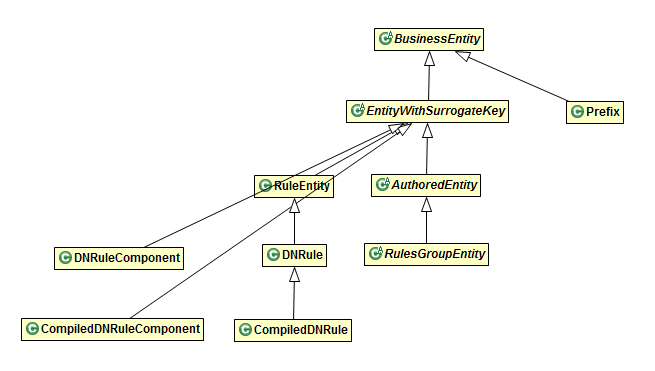
\includegraphics[width=0.8\textwidth]{images/dia-fe-bo.png}
    \caption{Selected BO classes used in \FE}
	\label{fig:feBO}
\end{figure}

Description of the most important BO classes follows:

\begin{description}[style=nextline,font=\ttfamily]
	\item[BusinessEntity] The base class for all BO classes. It provides no functionality and serves just as a common abstract parent.
	\item[EntityWithSurrogateKey] The base class for BO classes for all entities with surrogate primary keys. It only contains the \code{id} property.
	\item[AuthoredEntity] This interface serves as an abstract parent of all entities that track their authors.
	\item[Prefix] This BO represents an URI prefix. It maps to an internal Virtuoso relational table and it's structure is therefore fixed.
	\item[DNRule and DNRuleComponent] These entities represent DN rules and rule components and are useful when working with rules in the raw form.
	\item[CompiledDNRule and CompiledDNRuleComponent] These entities represent DN rules and rule components and are easier to use when working with rules compiled from template instances.
\end{description}

\subsubsection{dao}

This package (and it's subpackages) contains classes which form the DAO layer. See the related section for more information on that.

\subsubsection{core}

The \code{core} package contains \code{ODCSWebFrontendApplication} and \code{ODCSWebFrontentSession}\linebreak classes extending the standard Wicket classes representing a web application and session, respectively, and the \code{ODCSWebFrontendApplication.properties} file. The properties file contains custom validation messages and declarations of other string literals. In addition, the package contains the following items:

\begin{description}[style=nextline,font=\ttfamily]
	\item[URLRouter] Handles URL routing - e.g. conversion from raw Wicket-like URL addresses to human readable ones (and vice versa).
	\item[DaoLookupFactory] Encapsulates DB connections and serves DAO objects to page components (see Section \ref{sec:frontendDao}).
\end{description}

\subsubsection{core.models}

This package contains custom implementations of the \code{IDataProvider} and \code{SortableDataProvider} interfaces, which adhere to our DAO layer implementation.

\subsubsection{core.components}

In the \code{core.components} package you'll find several custom components, such as labels, buttons, etc. The following list describes some of them. For a more comperhensive description, please see the javadoc documentation.

\begin{description}[style=nextline,font=\ttfamily]
	\item[UnobtrusivePagingNavigator] An implementation of the \code{PagingNavigator} component which is not visible if the list contains only a single page.
	\item[TruncatedLabel] A label which only displays a few first characters of the given string.
	\item[TimestampLabel] A label to display a properly formated timestamp.
	\item[RedirectButton] A button to redirect to a different page, adjusted to suit the structure of the \FE application.
	\item[LogInPanel] A panel which contains the log-in form.
	\item[LimitedEditingForm] A form that can only be confirmed by authorized users.
	\item[HelpWindow] A generic modal window to display help information.
\end{description}

\subsubsection{pages}

In this package there are Wicket components for individual pages. The structure of subpackages mirrors the \FE menu. These are mostly standard Wicket components (but for a few conventions we have applied - read more in Section \ref{sec:howToAddANewPage}). In this section, a brief description of some of the non-standard components will be given.

\begin{description}[style=nextline,font=\ttfamily]
	\item[FrontendPage] The parent component for almost all (see below) page components. Provides page layout and content common to all pages, as well as factory methods to create some basic child components.
	\item[LogoutPage] This component does not extend \code{FrontendPage}, for it does not represent a proper page. It's purpose is to log out the current user and then redirect to home-page.
	\item[UserPanel] This component forms the user-information panel - it shows the username and list of roles of the currently logged in user and provides means to log-in and log-out. It is included as a child component in the \code{FrontendPage}.
\end{description}
	
For more information on how to create a new page, see Section \ref{sec:howToAddANewPage}.

\subsubsection{util}

This package is intended for \FE specific utility classes, such as classes to ease working with arrays (\code{ArrayUtils}), sending email messages (\code{Mail}, \code{NewAccountMail}, \code{NewPasswordMail}) and generating and hashing passwords (\code{PasswordHandling}) - to name some of them.

Some methods in other parts of the \FE codebase accept code snippets (e.g. closures) as arguments. Because the current version of Java (1.6) does not directly support closures, we have created two classes - \code{CodeSnippet} and \code{EmptyCodeSnippet} - to be used instead. They too belong in the \code{util} package.

\subsubsection{validators}

This package contains custom Wicket form validators, such as \code{IRIValidator} - ensures that the given value is a valid IRI, \code{EnumValidator} - ensures that the given value is an element of the represented enumeration or \code{OldPasswordValidator} - ensures that the given new password matches the original one.

All our custom validators extend the \code{CustomValidator} class, which handles error message propagation so that validators can focus just on the validation process.

\subsection{Database Access Layer}
\label{sec:frontendDao}
\FE has a layer for accessing the database based on Spring and its JDBC templates. We chose not to use Hibernate due to integration problems with Wicket and use custom implemenation of business and DAO objects.

Entities retrieved from database are represented by POJOs (Plain Old Java Objects). The code that actually retrieves them is in a DAO class, by convention having suffix \code{Dao} and inheriting from the base class \code{Dao}. DAO objects internally call methods of the Spring's \code{JdbcTemplate} and passes to it a class extending \code{CustomRowMapper} which implements creation of the POJO business object(s) from query results.

The DAO objects can be obtained from an instance of \code{DaoLookupFactory} (available e.g. as a protected member of \code{FrontendPage}). A DAO object can be obtained by calling a \code{getDao()} method which returns an existing DAO object or creates a new one if necessary. Signatures of \code{getDao()} methods are:

\begin{verbatim}
  public <T extends Dao> T getDao(Class<T> daoClass)
  public <T extends Dao> T getDao(Class<T> daoClass, boolean commitable)
\end{verbatim}

We utilize generics in Java to obtain a specific type of a DAO class. In addition, there may be two versions of a DAO class -- one for a read-only view of commited version of an entity and one for the working version visible only to the author (see Section \ref{sec:authorshipAuth}). One can use the second version of the \code{getDao()} method and request either the read-only or commitable version.

Commitable and read-only DAOs are implemented using a custom \code{@CommitableDao} annotation. The read-only version should be annotated with \code{@CommitableDao} having the commitable DAO class as its argument. The commitable version must inherit from the read-only DAO.

Hierarchy of DAO objects is depicted on \figurename~\ref{fig:feDAO}.

\begin{figure}[htb]
    \centering
    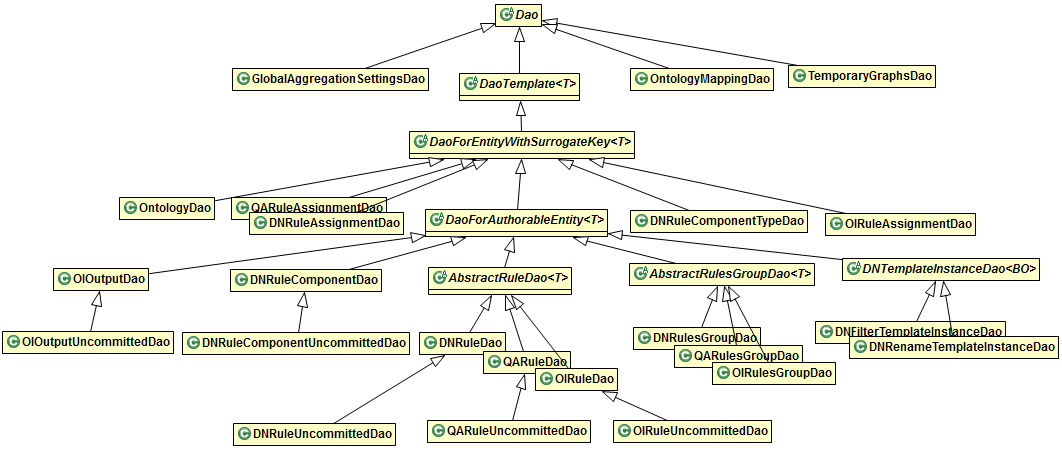
\includegraphics[width=1.05\textwidth]{images/dia-fe-dao.png}
    \caption{Selected DAO classes used in \FE}
	\label{fig:feDAO}
\end{figure}

\subsubsection{Important DAO Classes}
Description of the most important DAO classes follows:

\begin{description}[style=nextline,font=\ttfamily]
	\item[Dao] This is the base class of all DAO classes. It keeps an instance of \code{JdbcTemplate} and provides access to it either directly or through utility methods \code{jdbcQuery()}, \code{jdbcQueryForInt()}, \code{jdbcQueryForList()}, etc. It can also execute code in a Spring transaction with \code{executeInTransaction()} and handles proper recognition of some exceptions thrown by Virtuoso JDBC driver.
	\item[DaoTemplate] This method provides convenience methods for loading of one or more entities from the database. Its \code{getTableName()}, \code{getRowMapper()}, \code{getSelectAndFromClause()}, \code{postLoadAllBy()} and \code{postLoadBy()} methods can be used to customize the loading. Other methods are declared as final.
	\item[DaoForEntityWithSurrogateKey] This DAO is used for working with entities with a primary key. The corresponding business objects must inherit from \code{EntityWithSurrogateKey}. It extends \code{DaoTemplate} with additional methods for loading, deleting and saving an entity by its primary key.
	\item[DaoForAuthorableEntity] This class is intended for entities that can be edited only by their author. It adds an abstract method \code{getAuthorId()}.
	\item[AbstractRuleDao] Base class for (QA, DN, Linker) transformer rules. It provides methods for commiting of changes and disables any delete and update operations.
	\item[XXXRuleDao] Concrete classes inheriting from AbstractRuleDao. It can be used for read-only access to rules (their commited version, respectively). \code{save()} and \code{update()} methods throw an exception. It is annotated with \code{@CommittableDao(XXXRuleUncommittedDao.class)} so that the commitable/editable version can be obtained.

		An instance of this DAO may be obtained by calling e.g.\\
		\code{daoLookupFactory.getDao(XXXRuleDao, false)}.
	\item[XXXRuleUncommittedDao] These classes inherit from \code{XXXRuleDao} and provide the editable and commitable view on transformer rules. Changes may be commited in transaction by calling \code{commitChanges()}.

		An instance of this DAO may be obtained by calling e.g.\\
		\code{daoLookupFactory.getDao(XXXRuleDao, true)}.
	\item[OntologyDao] This class extends \code{DaoForEntityWithSurrogateKey} and is used for working with ontologies. When storing an ontology, firstly its definition is stored to a RDF graph, which's name is derive from ontology label. After that the ontology is stored to the relational database. This order is chosen to avoid using transaction across RDF and relation data, which does not work. Ontology definition is stored to the relational database as well to keep its formatting and possible comments. Finally quality assessment and data normalization rules are generated from stored ontology (see Sections \ref{sec:QA} and \ref{sec:DN}).
\end{description}

\subsection{Authorization}
There are two main scopes of authorization in \odcs -- authorization based on roles and authorization based on the authorship of an entity.

\subsubsection{Roles}
Authorization based on roles recognizes 5 roles: Administrator (ADM), Pipeline Creator (PIC), Ontology Creator (ONC), Data Producer (SCR) and Data Consumer (USR). Their detailed description is given in \refusermanual. Roles can be assigned to users in \FE and a user can have any number of roles.

We use means provided by Wicket to apply authorization by role. Pages and components can be marked with \code{@AuthorizeInstantiation} annotation with enumeration of roles that are required to access the page or component (at least one of the roles from the given list is required). The roles assigned to the currently logged-in user are kept in the session object \code{ODCSWebFrontendSession} which extends Wicket \code{AuthenticatedWebSession} for this purpose.

\subsubsection{Authorship}
\label{sec:authorshipAuth}
Authorization based on authorship is necessary for entities that can be only edited by their author. Rule groups and rules, for example, can be only edited by the user who created them or by user having the role Administrator. To facilitate checking of whether the current user is authorized for entity editing, class \code{LimitedEditingPage} extending \code{FrontendPage} was introduced.

\code{LimitedEditingPage} requires two additinal arguments in its constructor: edited entity ID and a DAO class for the authorable entity (\code{DaoForAuthorableEntity}), which can retrieve author based on entity ID. It then checks whether the current user is authorized using a helper class \code{AuthorizationHelper} and makes this information accessible with protected methods.

Every page that needs information about whether the user is authorized for editation of can call protected methods \code{checkUnauthorizedInstantiation()} to prevent the user from displaying the page or \code{isEditable()} to detect whether the user is authorized for editation.

Because transformer rules and related settings must be commited before the changes are visible to  users not 
authorized for editation (who have a read-only access to rules), there are two versions of rules in the database -- one version is visible for the author and Administrators (these tables have suffix \code{\_UNCOMMITED}) and one version visible for Engine and other users. The proper table version for the current user can be obtained by method \code{getVisibleTableVersion()}.

\code{}

\section{Extending}

\subsection{How to Add a New Page}
\label{sec:howToAddANewPage}

First of all make sure that you are familiar with the Wicket framework, for the whole web application is based on it.

A standard Wicket \code{WebPage} component is used to create new pages. That means that you can use all the standard stuff that Wicket provides, such as adding standard child components (forms, tables, links, ...). Aditionaly, you should adhere to some specific conventions, which have been established to ease and fasten the development process and to make the web well structured and consistent. This section provides you with details on these conventions.

The POJO part of the page component should extend the \code{FrontendPage} class. The \code{FrontendPage} component provides page layout and content for parts of the page which are common throughout the whole application (such as logo and menu bar). That's why, when creating a new page, you only need to take care of the custom content. There are two components handled by the \code{FrontendPage} which need per-page parameters - the page title and the bread crumbs. The newly created page should supply these values via a call to the constructor of the parent's class. The \code{FrontendPage} also contains several helper factory methods which can be used to construct simple child components. Last but not least, the \code{FrontendPage} provides two shortcut methods - \code{getApp()} to obtain the application object and \code{getODCSSession()} to get the session object. All of these are protected scoped and can be used arbitrarily in new page components.

The POJO must provide a constructor. The constructor should be either parameter-less or accept a single parameter -- the id of entity to be described on the page. Inside the constructor you generaly need to call the parent's constructor (and suply the page title and crumbs values), obtain all needed DAO objects via the \code{daoLookupFactory} class attribute (see Section \ref{sec:frontendDao} ) and add all child components, ideally through calls to private methods, one for each component.

You will also want to update the HTML file of the \code{FrontendPage} component in order to add a link to the new page to the menu bar. Simply add a new standard Wicket link to the HTML list.

All parts of the web frontend application adhere to the following structure rules. Every section describes registered entities of a single type (such as transformers, pipelines, ontologies, user accounts). For every entity type (say XXX) there are four page components - \code{XXXListPage} (shows a list of all registered entities), \code{NewXXXPage} (provides a form to register a new entity), \code{XXXDetailPage} (shows an existing entity in details and provides a form to edit it; if there are subentities bound to the entity then shows a list of all of them).

As a rule, every page should contain a single help pop-up window for every entity the user can work with via that page. To create a help pop-up window for a new entity type (say XXX again), you only need to create an XXXHelpPanel component (you can copy an existing help panel component and update the contents in the related HTML page). Then use the \code{addHelpWindow} method of the \code{FrontendPage} class to add the pop-up window to the page.


\subsection{How to Add a New \DN Template}
\label{sec:howToAddANewDNTemplate}

To add a new \DN Template (named say XXX, such as Filter, Rename, Replace), follow these steps.

Create a new relational table in the Virtuoso database. The table should be named \code{DB.ODCLEANSTORE.DN\_XXX\_TEMPLATE\_INSTANCES} and contain \code{id} as a surrogate primary key, \code{groupId} as a foreign key which points to the group of rules to which the template instance belongs, \code{rawRuleId} as a foreign key which points to the raw version of the represented rule and columns for attributes of the template.

Add a new Business Object to the \code{cz.cuni.mff.odcleanstore.webfrontend.bo.dn} package named \code{DNXXXTemplateInstance}. The class should adhere to standard BO conventions (see the relevant section) and relate to the table created in the previous step.

Add a compiler class to the same package called \code{DNXXXTemplateInstanceCompiler}. It must extend the \code{DNTemplateInstanceCompiler<DNXXXTemplateInstance>} class and override the \code{compile} method. This methods accepts an \code{DNXXXTemplateInstance} instance as a parameter and compiles it into a standard \code{CompiledDNRule} instance (e.g. into a raw rule form), which it then returns.

Add a new section to the \code{DNGroupDetailPage} component and implement the \linebreak\code{NewDNXXXTemplateInstancePage} and \code{EditDNXXXTemplateInstancePage} components. You will also need to add the \code{DNXXXTemplateInstanceHelpPanel} and use it as a pop-up help window. Fore a more detailed explanation of this step, see Section \ref{sec:howToAddANewPage}.

Note that when implementing a new DN template type it is a good idea to copy and rename the classes which belong to an existing one and just overwrite the template specific parts.



%%%%%%%%%%%%%%%%%%%%%%%%%%%%%%%%%%%%%%%%%%%%%%%%%%%%%%%%%%%%%%%%%%%%%%%%%%%%%%
\chapter{Future Work}
\odcs could be extended in many ways. Suggestions for future work and improvements are maintained at a dedicated page\footnote{\url{https://sourceforge.net/p/odcleanstore/wiki/Future\%20extensions/}} at project website. This chapter lists the most important ideas for future work. Items in bold should be implemented in future and were omitted for time reasons.

\section{Data Processing}
\begin{itemize}
	\item Improved logging. As of now, There is one log file for Engine and a dedicated log file for each transformer instance. In addition, some information about Engine is updated in the relational database. However, structured logs in the database for transformers (e.g. with information about transformer instance, pipeline, its author etc.) may improve usage for both pipeline creators and transformer creators.
	\item Quarantine. Data that are considered suspicious (e.g. having too low \QA score) would be moved to an isolated dataspace where it would wait to be checked by an administrator and then accepted, corrected or deleted.
	\item Possibility to review data and modify it from a user interface. An advanced extension would be possibility to modify multiple named graphs in a batch operation. The provenance information for affected graphs should contain information about editing.
	\item Transformer that would detect identical update of a named graph already stored in the database and would only update metadata of the stored graph instead of storing both copies.
	\item Store the original unprocessed version of data so that the original version can be used again when a pipeline damages the data.
	\item Automatically download missing ontologies used in processed data.
	\item \textbf{Introduce concept of \quot{post-transformers}} that would be run on data \textit{after} they are processed by a pipeline and moved to the clean database. They could be used e.g. for updating data in the clean database depending on stored graphs, such as what Quality Aggregator does.
\end{itemize}

\section{\QA}
\begin{itemize}
	\item Track more quality dimensions (e.g. completnes, timeliness).
	\item Machine learning. Rules could be derived from a given set of named graphs and their scores.
\end{itemize}

\section{\DN}
\begin{itemize}
	\item More rule templates, improved administration in case there would be too many templates.
\end{itemize}

\section{Output Webservice \& \CR}
\begin{itemize}
 	\item Support queries for any SPARQL (CONSTRUCT) (not only the current URI, keyword and named graph query). This is a more complex extension as \CR would need to be able to load metadata and \code{owl:sameAs} links by itself and moreover efficiently.
	\item Paging of results.
	\item Sorting of results of a keyword query by relevance for the given keyword.
	\item Add query which would return all resources of the given \code{rdf:type}.
	\item Generalize the interface for passing metadata to \CR. As of now, there is an exactly defined set of metadata that are accepted by \CR which limits extending.
	\item More customizable \aggrq computation. For example, the user could have the possibility to specify how much she trusts each publisher and the \aggrq would take that into consideration.
	\item More aggregation methods, such as TOP-K -- K best values. This would require the possibility to parametrize aggregation methods.
\end{itemize}

\section{\FE}
\begin{itemize}
	\item \textbf{The possibility to create a custom (deep) copy of an arbitrary group of rules.}
	\item \textbf{The possibility to create a custom copy of a rule.}
	\item \textbf{The possibility to create a custom copy of a pipeline.}
	\item \textbf{Labels and descriptions for transformer instances.}
	\item Filtering of entities displayed in \FE by values for each column. Possibility to show only entities created by the current user.
	\item Notification about changes in a rule group. If the author of a rule group modifies it, a notification would be sent to all users whose pipelines use the rule group and they would be provided with the option to accept of refuse the changes (would require versioning of rule groups or cloning of rule groups.).
	\item Transformer instance templates. It would be possible to assign a pre-prepared transformer instance to a pipeline which could contain transformer configuration, assigned rule groups etc.
	\item Possibility to upload a .jar archive containing a transformer directly through \FE.
	\item Possibility to run affected pipelines when a rule group is deleted.
	\item Show list of affected pipelines for a rule group or transformer.
	\item Check syntactical validity of rules when they are entered. Could be implemented by running the rule on an empty testing graph and checking for an error.
\end{itemize}

\section{Miscellaneous}
\begin{itemize}
	\item \textbf{Installer will be able to install Engine as a system service on Windows or a daemon on Linux, respectively.}
	\item Provide a tool (command line or with GUI) for import of large graphs. \odcs is designed mainly for processing of smaller graphs (e.g. results of \QA might not be relevant for too large graphs). A large graph could be divided into multiple small graphs and sent to Input Webservice in parts.
\end{itemize}

\section{Known Issues}
\begin{itemize}
	\item Non-ASCII characters may get broken when entered into certain fields (descriptions, ontology definitions) in \FE. This is caused by incompatibility of  Spring's JdbcTemplate and Virtuoso.
	
\end{itemize}

%%%%%%%%%%%%%%%%%%%%%%%%%%%%%%%%%%%%%%%%%%%%%%%%%%%%%%%%%%%%%%%%%%%%%%%%%%%%%%
\chapter{Related Work}
\label{chap:relatedWork}
\odcs provides means for cleaning, linking, and scoring incoming RDF data, storing it, and provides aggregated and integrated views on the data to Linked Data consumers. In addition, we support trustworthiness of the data with aggregate quality and provenance tracking. 

\odcs focuses on the data processing and queries over stored data. Nevertheless, the extraction process that feeds data to  \odcs is also important -- our sister project Strigil implements a web scraper and document extractor that produces RDF data and integrates with ODCleanStore for storing the produced data.

\section{Data Extraction}


\subsection*{Strigil}

Strigil\footnote{\url{http://sourceforge.net/p/strigil/home/Home/}} implements a web scraper and document extractor that produces RDF data and integrates with ODCleanStore as the producer of data.

\subsection*{Linked Data Manager}
Linked Data Manager\footnote{\url{http://www.semantic-web.at/linked-data-manager}} (LDM) is a Java based Linked (Open) Data Management Suite to schedule and monitor required Extract - Transform - Load jobs for web-based Linked Open Data portals as well as for sustainable Data Management and Data Integration usage.

LDM data processing pipeline is similar to the data processing pipeline in ODCleanStore. LDM is a counterpart of ODCleanStore in that it provides facilities for managing the extraction process but doesn't provide any permanent storage or direct access to the data. Thus an LDM Loader could be used to send data to ODCleanStore and access it from here.

\section{Data Processing}

\subsection*{Linked Data Integration Framework}
Linked Data Integration Framework\footnote{\url{http://www4.wiwiss.fu-berlin.de/bizer/ldif/}} (LDIF) is an open-source Linked Data Integration Framework that can be used by Linked Data applications to translate Web data and normalize URI while keeping track of data provenance.
The framework consists of a Scheduler, Data Import and an Integration component with a set of pluggable modules.

LDIF components encompass the whole process from data import and processing to integration and quality assessment. We use some of LDIF componets internally in ODCleanStore (Silk). The main difference is that LDIF is a framework other applications can built on, while ODCleanStore is a ready-to-use solution that can be easily deployed and managed via a web interface. Differences in quality assessment and data aggregation with Sieve, a part of the LDIF framework, are described below. LDIF also supports provenance tracking.\footnote{See Figure 2 of \href{http://static.lod2.eu/Deliverables/deliverable-4.3.2.pdf}{LOD2 Deliverable 4.3.2}}

\section{Data aggregation and quality}

\subsection*{Sieve}
Sieve\footnote{\url{http://sieve.wbsg.de/}} adds quality assessment and data fusion capabilities to the LDIF architecture. It uses metadata about named graphs in order to assess data quality, agnostic to provenance vocabulary and quality models. Sieve uses customizable scoring functions to output data quality descriptors. Based on these quality descriptors (and/or optionally other descriptors ), Sieve can use configurable FusionFunctions to clean the data according to task-specific requirements.

Sieve offers functionality similar to our Conflict Resolution component; however the purpose of Sieve in LDIF is different - it aggregates data while being stored to the clean database (unlike Conflict Resolution used at query time). This may be suitable when the desired data are known in advance but is not sufficient for open Web environments, where every consumer has different requirements on the aggregated data. Furthermore, ODCleanStore provides quality for each result statement where Sieve computes quality only for whole named graph.

\subsection*{Integration systems in relational databases}

The problem of integration of heterogeneous data (solved in ODCleanStore for RDF data) is solved by several systems for relational databases, e.g. Aurora\footnote{\url{http://citeseerx.ist.psu.edu/viewdoc/summary?doi=10.1.1.50.7261}} or Fusionplex\footnote{\url{http://dl.acm.org/citation.cfm?id=1221048}}.


Aurora is an integration system of heterogenous data residing in relational and object-oriented databases, i.e. deals with non-RDF data; its query model enriches the SQL SELECT by enabling to define attribute conflict resolution functions (e.g. age[ANY] means that any attribute value for  the attribute age is used in the query) and record conflict  resolution function, which deal with key attributes of the records.   ODCS offers more built-in aggregation methods, on the other hand, Aurora allows user defined attribute aggregation functions; in ODCS, record conflicts are either discovered by linkers, or there is no record conflict.

%%%%%%%%%%%%%%%%%%%%%%%%%%%%%%%%%%%%%%%%%%%%%%%%%%%%%%%%%%%%%%%%%%%%%%%%%%%%%%
\chapter{Conclusion}
The goal of the project was to build a server application that would automate processing -- especially cleaning, linking and scoring -- of data in RDF format and provide aggregated and integrated views on the processed data to Linked Data consumers. We have successfully implemented all these features in \odcs and hope that the project will continue to be used and developed.

\odcs brings several contributions. There are other tools for RDF data processing (see related work in Chapter~\ref{chap:relatedWork}) but they are mostly frameworks that other developers can build on. \odcs was developed as a whole solution that can be readily deployed and used. It ships with an web administration interface so that all neccessary configuration can be done in a web browser. It should be noted, however, that administrators of \odcs should have some technical knowledge -- at least understand RDF and SPARQL query language.

Another novel aspect is provenance tracking and data fusion/conflict resolution. This feature should support addoption of Linked Data by justifying why users should (or shouldn't) believe the data they are presented and where they can verify it and thus increase trust in Linked Data. Unlike other solutions, \odcs solves conflicts at query time which is suitable for the open Web environment where every consumer may have different requirements.

We hope that \odcs will provide basis for further work with Linked Data and other developers will extend it and customize it for their own purposes. We introduced the concept of pluggable transformers so that whatever functionality is needed can be added.

Several papers about \odcs were accepted at scientific conferences. The reception was positive and we used the feedback to improve our project. In addition, \odcs was evaluated on real data, e.g. data extracted from information system for public contracts\footnote{\url{http://www.isvzus.cz/}} run by the Ministry of Regional Development in the Czech Republic. We also used the feedback to improve our project and adapt it to a real-world use case.

We hope that \odcs will prove to be a useful tool for RDF data processing and will contribute to adoption of Linked Data. It was designed as a general tool for Linked Data management with basic data processing capabilities. We hope that the development will continue, new uses for \odcs will emerge and the project will be extended and customized for the particular use cases.



%%%%%%%%%%%%%%%%%%%%%%%%%%%%%%%%%%%%%%%%%%%%%%%%%%%%%%%%%%%%%%%%%%%%%%%%%%%%%%

\appendix

%%%%%%%%%%%%%%%%%%%%%%%%%%%%%%%%%%%%%%%%%%%%%%%%%%%%%%%%%%%%%%%%%%%%%%%%%%%%%%
\chapter{Glossary}
\label{chap:glossary}
\section*{RDF-related}
\begin{glossarylist}
	\item[RDF] Resource Description Framework, a~language for representing information about resources in the World Wide Web\footnote{\url{http://www.w3.org/RDF/}}
	\item[RDF triple] Statement about a~resource expressed in the form of subject-predicate-object expression
	\item[URI] Uniform Resource Identifier, identifies RDF resources
	\item[Named graph] A~set of related RDF triples (RDF graph) named with a~URI\footnote{\url{http://www.w3.org/2004/03/trix/}}
	\item[RDF quad] An RDF triple plus named graph URI (subject, predicate, object, named graph)
	\item[Ontology] Representation of the meaning of terms in a~vocabulary and of their interrelationships
	\item[OWL] The Web Ontology Language\footnote{\url{http://www.w3.org/TR/owl-features/}}
	\item[SPARQL] RDF query language\footnote{\url{http://www.w3.org/TR/rdf-sparql-query/}}
	\item[RDF/XML] An XML-based serialization format for RDF graphs\footnote{\url{http://www.w3.org/TR/rdf-syntax-grammar/}}
	\item[TTL] Turtle -- Terse RDF Triple Language\footnote{\url{http://www.w3.org/TeamSubmission/turtle/}}; a~human-friendly alternative to RDF/XML 
\end{glossarylist}

\section*{Data \& Data Quality}
\begin{glossarylist}
	\item[Dirty (staging) database] Database where incoming data are stored until they are processed by a~processing pipeline (e.g. clean, linked to other data, etc.)
	\item[Clean database] Database where incoming data are stored after they are successfully processed by the respective processing pipeline; this database can be accessed using the Output Webservice
	\item[\code{Payload} graph] Named graph where the actual inserted data, given in the \code{payload} parameter of Input Webservice, are stored
	\item[\code{Provenance} graph] Named graph where additional provenance metadata, given in the \code{provenance} field of Input Web Service, are stored
	\item[Metadata graph] Named graph where other metadata about a \code{payload} graph (such as source, timestamp, license, etc.) are stored
	\item[Attached graph] Named graph attached to a \code{payload} graph by a transformer
	\item[Named graph score] Quality of a~single (\code{payload}) named graph estimated by the Quality Assesment component and stored in the database, expressed as a~number from interval [0,1]
	\item[Publisher score] Average score of named graphs from a~publisher
	\item[Aggregate quality] Quality of a~triple in the results calculated by the Conflict Resolution component during query time, expressed as a~number from interval [0,1]
\end{glossarylist}

\section*{Data Processing}
\begin{glossarylist}
	\item[Pipeline] A configurable sequence of transformers that is used to process a named graph. The pipeline to process data sent to Input Webservice can be selected explicitly, or the default pipeline is used.
	\item[Transformer] A Java class which implements the \term{Transformer} interface that and is registered in ODCleanStore Administration Frontend by an administrator.
	\item[Transformer instance (or transformer assignment)]  Assignment of a \term{transformer} to a \term{pipeline}. A single transformer can be assigned to multiple pipelines (or even to a single pipeline multiple times), thus creating multiple transformer instances.
	\item[Rule] Some transformers included in ODCleanStore can be configured in Administration Frontend by rules. Rules are grouped together to \term{rule groups}.
	\item[Rule group] A group of transformer \term{rules}. Rule groups can be assigned to transformer instances.
\end{glossarylist}

\section*{User Roles}
\begin{glossarylist}
	\item[ADM] Administrator
	\item[ONC] Ontology creator
	\item[PIC] Pipeline creator
	\item[SCR] Data producer (scraper)
	\item[USR] Data consumer
\end{glossarylist}

%%%%%%%%%%%%%%%%%%%%%%%%%%%%%%%%%%%%%%%%%%%%%%%%%%%%%%%%%%%%%%%%%%%%%%%%%%%%%%
%\chapter{ODCS ontology}

%%%%%%%%%%%%%%%%%%%%%%%%%%%%%%%%%%%%%%%%%%%%%%%%%%%%%%%%%%%%%%%%%%%%%%%%%%%%%%
\chapter{Relational Database Schema}
\label{chap:reldb}

\begin{figure}[htbp]
    \centering
    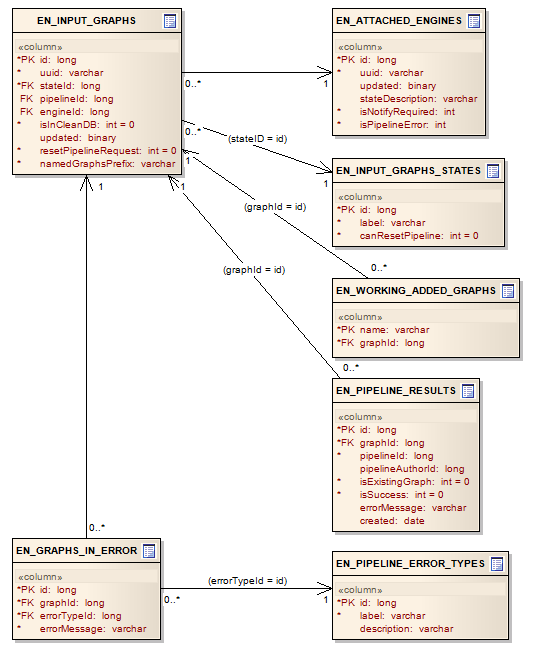
\includegraphics[scale=0.6]{images/db-engine.png}
    \caption{Diagrams of database tables related to Engine}
	\label{fig:dbEngine}
\end{figure}

\begin{figure}[htbp]
    \centering
    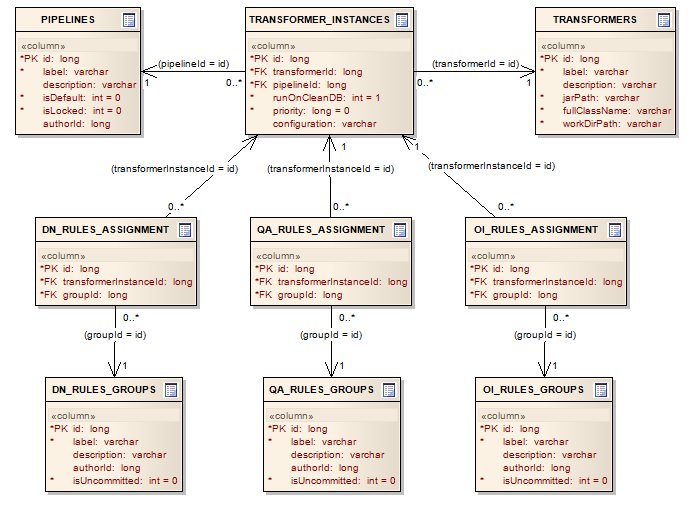
\includegraphics[scale=0.6]{images/db-pipelines.png}
    \caption{Diagrams of database tables related to pipelines}
	\label{fig:dbPipelines}
\end{figure}

\begin{figure}[htbp]
    \centering
    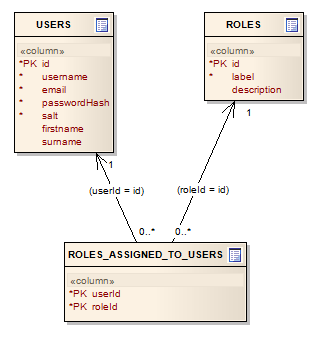
\includegraphics[scale=0.6]{images/db-fe.png}
    \caption{Diagrams of database tables related to \FE}
	\label{fig:dbFrontend}
\end{figure}

\begin{figure}[htbp]
    \centering
    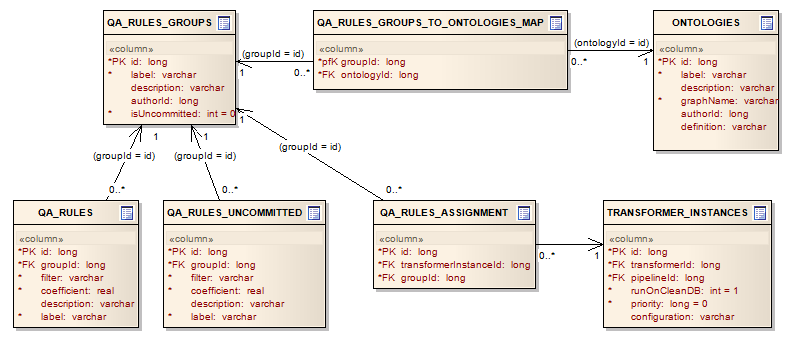
\includegraphics[scale=0.6]{images/db-qa.png}
    \caption{Diagrams of database tables related to \QA}
	\label{fig:dbQA}
\end{figure}

\begin{figure}[htbp]
    \centering
    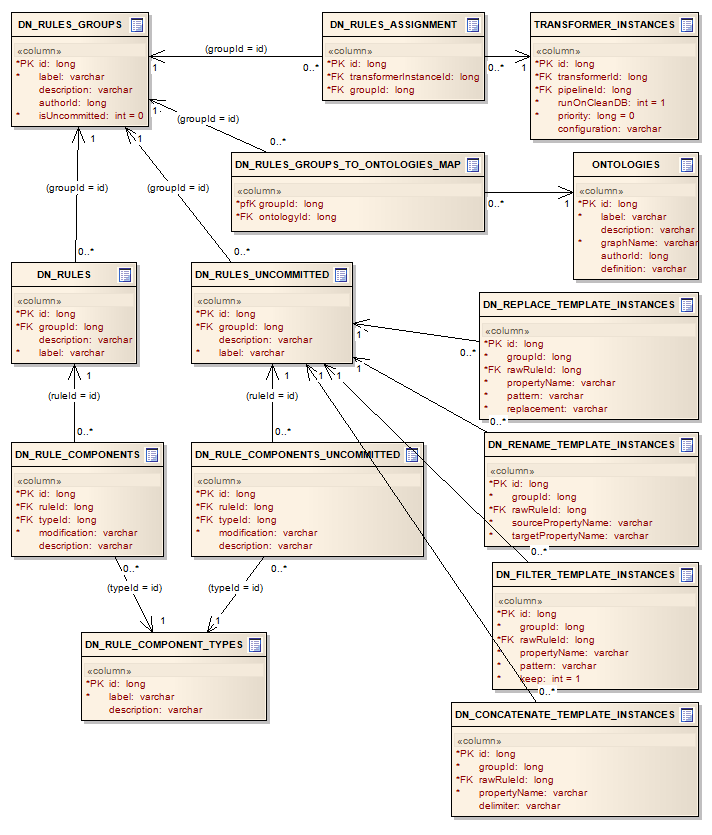
\includegraphics[scale=0.6]{images/db-dn.png}
    \caption{Diagrams of database tables related to \DN}
	\label{fig:dbDN}
\end{figure}

\begin{figure}[htbp]
    \centering
    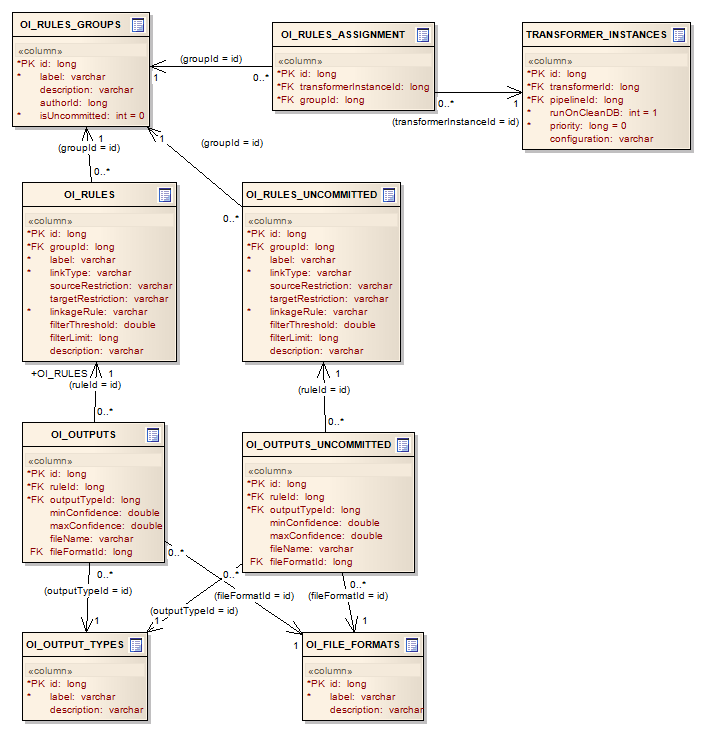
\includegraphics[scale=0.6]{images/db-oi.png}
    \caption{Diagrams of database tables related to \OI}
	\label{fig:dbOI}
\end{figure}

\begin{figure}[htbp]
    \centering
    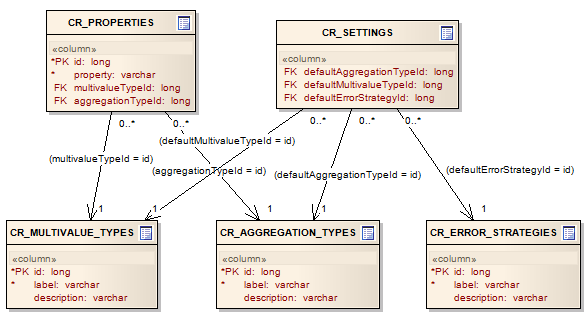
\includegraphics[scale=0.6]{images/db-cr.png}
    \caption{Diagrams of database tables related to \CR}
	\label{fig:dbCR}
\end{figure}

\begin{figure}[htbp]
    \centering
    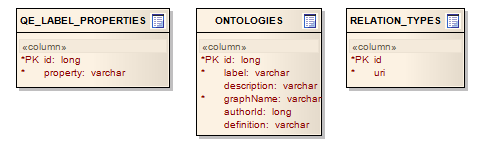
\includegraphics[scale=0.6]{images/db-misc.png}
    \caption{Diagrams of miscellaneous database tables}
	\label{fig:dbMisc}
\end{figure}

%%%%%%%%%%%%%%%%%%%%%%%%%%%%%%%%%%%%%%%%%%%%%%%%%%%%%%%%%%%%%%%%%%%%%%%%%%%%%%
\chapter{List of Used XML Namespaces}
\begin{table}[h!]
\centering
\begin{tabular}{|l|l|}
	\hline
	\ttfamily
	\textrm{\textbf{Prefix}} & \textrm{\textbf{URI}} \\
	\hline\hline
	odcs & http://opendata.cz/infrastructure/odcleanstore/ \\
	\hline
	w3p & http://purl.org/provenance\# \\
	\hline
	dc & http://purl.org/dc/terms/ \\
	\hline
	rdf & http://www.w3.org/1999/02/22-rdf-syntax-ns\# \\
	\hline
	rdfs & http://www.w3.org/2000/01/rdf-schema\# \\
	\hline
	owl & http://www.w3.org/2002/07/owl\# \\
	\hline
	xsd & http://www.w3.org/2001/XMLSchema\# \\
	\hline
	dbpedia & http://dbpedia.org/resource/ \\
	\hline
	dbprop & http://dbpedia.org/property/ \\
	\hline
	skos & http://www.w3.org/2004/02/skos/core\# \\
	\hline
\end{tabular}
\caption{List of used XML namespaces}
\end{table} 

%%%%%%%%%%%%%%%%%%%%%%%%%%%%%%%%%%%%%%%%%%%%%%%%%%%%%%%%%%%%%%%%%%%%%%%%%%%%%%
%\chapter{Project organization}

%begin{itemize}
	%\item Team, task division (Developer-Component-Main responsibilities)
	%\item Meetings
	%\item Release process (+ presentation)
	%\item Remarks?
%\end{itemize}

\end{document}
